%% Master Thesis : American University of Beirut
%% May 5, 2014
%% Mohamad Noureddine <man17@mail.aub.edu>

\documentclass[12pt, twoside, a4paper]{report}

\textheight23cm \textwidth16cm

%_________________________________________________________%
%\usepackage[dvips]{graphicx}
%\usepackage{latexsym}
%\usepackage{epsf}
%\usepackage{epsfig}
%\usepackage{a4}
%
%\usepackage{amsmath} % real numbers, natural numbers, ...
%\usepackage{amssymb}
%\usepackage{amsthm}  % used for theorems and definitions 
%\usepackage{amsxtra}
%\usepackage{amsxtra}
%\usepackage{amsfonts}
%
%\usepackage{fancyhdr}
%\usepackage{tocbibind} %bibliography in the table of contents
%\usepackage{enumerate}
%\usepackage{amsthm}
%\usepackage{amsbsy}
%
%\usepackage{tikz}
%
%\usepackage{booktabs}
%\usepackage{paralist}
%
%\usepackage{algorithm}
%\usepackage{algpseudocode}
%
%\usepackage{graphics}
%\usepackage{color}
%%\usepackage[usenames,dvipsnames]{xcolor}
%\usepackage{graphicx}
%\usepackage{enumerate}
%\usepackage{fancyvrb}
%%\usepackage{alltt}
%\usepackage{url}
%
%\usepackage{colortbl}
%\usepackage{multirow}
%\usepackage{chngpage}
%\usepackage{tabularx}
%
%\usepackage{amsfonts}
%\newcommand{\Yes}{\checkmark}
%\usepackage{pifont}
%\newcommand{\No}{\hspace{1pt}\ding{55}}
%
%\usepackage{relsize}
%\include{geometry}

\newcommand{\cci}[1]{\texttt{#1}}

\newcommand{\Data}{\mathrm{Data}}
\newcommand{\func}{\mathit{func}}
\newcommand{\port}{\mathit{port}}
\newcommand{\export}{\mathit{export}}

\newcommand{\guard}{\mathit{guard}}
\newcommand{\source}{\mathit{src}}
\newcommand{\dest}{\mathit{dest}}

\newcommand{\ignore}[1]{}
\newcommand{\ie}{i.e.,}
\newcommand{\secref}[1]{Section~\ref{#1}}
\newcommand{\figref}[1]{Fig.~\ref{#1}}
\newcommand{\defas}{\stackrel{\mathrm{\scriptscriptstyle def}}{=}}

\newcommand{\true}{\ensuremath{\mathtt{true}}\xspace}
\newcommand{\false}{\ensuremath{\mathtt{false}}\xspace}
\newcommand{\goesto}[1][]{\stackrel{#1}{\longrightarrow}} % -->

\newcommand{\valu}[1]{\mathbf{#1}}




%% formulae
\newcommand{\Pm}{\ensuremath{\mathcal{S}}\xspace}         % program
\newcommand{\Sp}{\ensuremath{\mathcal{S}}\xspace}         % specification
\newcommand{\cfor}[1]{\MATH{\mathit{cfor}[#1]}}               % correction formula for inadequate vocabulary
\newcommand{\for}[1]{\MATH{\mathit{fm}(#1)}}                     % formula corresponding to an assignment
\newcommand{\Fo}{\ensuremath{\mathcal{F}}\xspace}
\newcommand{\Pre}{\ensuremath{\mathcal{P}}}                                % precondition
\newcommand{\Post}{\ensuremath{\mathcal{Q}}}                              % postcondition

%% tool
\newcommand{\mytool}{\ensuremath{\{\mathcal{P}\}\mathcal{S}\{\mathcal{Q}\}}} % the name of our tool
\newcommand{\caig}{\ensuremath{\mathcal{OLP}}\xspace}
\newcommand{\biptool}{\ensuremath{\mathcal{BIP\{I\}}}}
\newcommand{\psqlanguage}{\ensuremath{\mathcal{T}iny}}
\newcommand{\aigcircuit}{\ensuremath{\mathcal{C}}}

\newcommand{\lft}{\ensuremath{\mathcal{left}}\xspace}
\newcommand{\rgt}{\ensuremath{\mathcal{right}}\xspace}
\newcommand{\eina}{\ensuremath{\mathcal{eina}}\xspace}



%%%%%%%%%%%%%%%%%%%%%%% GENERAL MATH SYMBOLS %%%%%%%%%%%%%%%%%%%%%%%%%%%%%%

\newcommand{\Adj}{\mathop{\rm Adj}\nolimits}
\newcommand{\abs}[1]{\left| #1\right|}
\newcommand{\card}[1]{\left| #1\right|}
\newcommand{\ar}{\rightarrow}
%\newcommand{\ar}{\longrightarrow}
\newcommand{\al}{\alpha}
\renewcommand{\b}[1]{\overline{#1}}
\newcommand{\cat}{\mathbin{\frown}}
\newcommand{\choice}{\mbox{$[\hspace*{-1.0pt}]$}}
\newcommand{\ceil}[1]{\left\lceil #1 \right\rceil}
\renewcommand{\d}{\, . \,}      % separator in quantified formulae
\newcommand{\df}{\triangleq}
%\newcommand{\df}{\mbox{$\:\stackrel{\rm df}{=\!\!=}\:$}}
\newcommand{\dn}{\mbox{$\hspace{-0.1em}\downarrow\hspace{-0.1em}$}}
\newcommand{\Ex}{\mathop{\rm Ex}}
\newcommand{\es}{``"}   %empty string
\newcommand{\expect}[1]{{\rm E}\left[ #1 \right]}
\newcommand{\expectsq}[1]{{\rm E}^2\left[ #1 \right]}
\newcommand{\floor}[1]{\left\lfloor #1 \right\rfloor}
\renewcommand{\ge}{\geqslant}
\newcommand{\given}{\mid}
\newcommand{\halfind}{\hspace*{1.5em}}
\newcommand{\ifof}{\Longleftrightarrow} % logical equivalence
\newcommand{\img}{\mathrm{Image}}
\newcommand{\ints}{\cap}
\renewcommand{\l}{\ell}
\newcommand{\la}[1]{\mbox{$\, \stackrel{#1}{\rightarrow} \,$}}
\renewcommand{\le}{\leqslant}
\newcommand{\lra}{\mbox{$\longrightarrow$}}
%\newcommand{\mod}{\ \mathrm{mod}\ }
\newcommand{\oneton}{\{1,\,\ldots, n\}}
\newcommand{\n}{\ensuremath{[1:n]}} 
\newcommand{\paren}[1]{\left( #1 \right)}
\newcommand{\pair}[2]{\ensuremath{(#1, #2)}}
\newcommand{\pind}{\hspace*{3.0em}}
\newcommand{\pj}{\!\upharpoonright\!}
\newcommand{\proj}{\pj}
\newcommand{\preimg}{\mathrm{PreImage}}
\newcommand{\pl}{\!\parallel\!}
\newcommand{\s}{\mbox{$\hspace{-1pt}-\hspace{-2pt}$}}
\newcommand{\set}[1]{\ensuremath{\{ #1 \}}\xspace}
%\newcommand{\set}[1]{\{#1\}}
\newcommand{\seq}{\approx}
\newcommand{\spc}{\mbox{\vspace{-0.25in}}}
\newcommand{\stt}{\ | \ }
%\newcommand{\st}[1]{\ensuremath{[ #1 ]}\xspace}
\newcommand{\sub}{\subseteq}
\newcommand{\twodots}{\mathinner{\ldotp\ldotp}}
\newcommand{\tiff}{\textup{\ iff\ }}
\newcommand{\tl}[1]{\mbox{$\tilde{#1}$}}% abbreviated tilde
\newcommand{\tpl}[1]{\ensuremath{\langle #1 \rangle}}
\newcommand{\un}{\cup}
\newcommand{\union}{\bigcup}
\newcommand{\up}{\mbox{$\hspace{-0.1em}\uparrow\hspace{-0.1em}$}}
\newcommand{\Var}{\mathop{\rm Var}\nolimits}
\newcommand{\variance}[1]{{\rm Var}\left[ #1 \right]}
\newcommand{\w}{\omega}


%%%%%%%%%%%%%%%%%%% Ints, Reals, etc %%%%%%%%%%%%%%%%%%%%%%%%%%%%%

\newcommand{\reals}{{\mathbb R}}
\newcommand{\integers}{{\mathbb Z}}
\newcommand{\naturals}{{\mathbb N}}
\newcommand{\nat}{\naturals}
\newcommand{\nats}{\naturals}
\newcommand{\rationals}{{\mathbb Q}}
\newcommand{\complex}{{\mathbb C}}
\newcommand{\complexes}{{\mathbb C}}
\newcommand{\prob}{\ensuremath{\Pm \sat \pair{\Pre}{\Post}|_b }}


%%%%%%%%%%%%%%%%%%%%%%% Hoare Logic Symbols
\newcommand{\lng}{\langle}
\newcommand{\ra}{\rangle}
\newcommand{\htp}[3]{\ensuremath{\{#1\}\,#2\,\{#3\}}}
\newcommand{\htptc}[3]{\ensuremath{\langle#1\rangle\,#2\,\langle#3\rangle}}
\newcommand{\var}{\ensuremath{\varphi}}

\newcommand{\as}[1]{\ensuremath{\{#1\}}}               % partial correctness asserion
%\newcommand{\ts}[1]{\ensuremath{\langle #1 \rangle}}   % termination correctness asserion

\newcommand{\ch}{\mbox{[\hspace{-0.15ex}]}}

\newcommand{\pa}[1]{\{\ensuremath{#1}\}}
%\newcommand{\ta}[1]{$<$#1$>$}
\newcommand{\ta}[1]{$\langle$\ensuremath{#1}$\rangle$}

\newcommand{\pre}[1]{\textsf{Precondition: #1}}
\newcommand{\post}[1]{\textsf{Postcondition: #1}}

\newcommand{\satt}{\equiv}
\newcommand{\sat}{\models}
\newcommand{\satf}{\mbox{\ensuremath{=\hspace*{-5pt}|}}}   % satisfiable - backward turnstile
%\newcommand{\satf}{\mbox{\ensuremath{=\!\!\!\!|}}}   % satisfiable - backward turnstile


\newcommand{\yld}{\vdash}
\newcommand{\yldd}{\equiv}
%\newcommand{\yldd}{\dashv \vdash}




\newcommand{\pc}[1]{{#1}}    %% font for pseudocode
%\newcommand{\pc}[1]{\codetext{#1}}    %% font for pseudocode



%%%%%%%%%%%%%%%%%%%%%%%% Lists
\newcommand{\be}{\begin{itemize}}
\newcommand{\ee}{\end{itemize}}
\newcommand{\bdn}{\begin{description}}
\newcommand{\edn}{\end{description}}
\newcommand{\bn}{\begin{enumerate}}
\newcommand{\en}{\end{enumerate}}
\renewcommand{\i}{\item}

\newenvironment{closeitemize}{\begin{list}%
{$\bullet$}%
{\setlength{\itemsep}{-0.2\baselineskip}%
\setlength{\topsep}{0.2\baselineskip}}}%
{\end{list}}



%\usepackage[square, comma, sort&compress]{natbib}

\setlength{\parindent}{1.5cm} % no paragraph indent

%%%%%%%%%%%%%%%%%%%%%%%%%%%%%%%%%%%%%%%%%%%%%%%%%%%%%%%%%%%
%%%%%%%%%%%%%%%%%%%%%%%%%%%%%%%%%%%%%%%%%%%%%%%%%%%%%%%%%%%
%%%%%%%%%%%%%%%%%%%%%%%%%%%%%%%%%%%%%%%%%%%%%%%%%%%%%%%%%%%
%% Thesis starts here!
\begin{document}

%_________________________________________________________%
\pagestyle{empty}
%------------------------------- TITLE PAGE(S) ------------------------------------------%
\begin{titlepage}
%\vspace{-1cm}
\begin{center}



\LARGE{AMERICAN UNIVERSITY OF BEIRUT\\} \vspace{3cm}

%%TODO: Modify the thesis tile to a better one. 
\LARGE{Verification of Software and Embedded Systems using AIG Solvers}
\vspace{3cm}



\normalsize{by\\} \Large{MOHAMAD ALI NOUREDDINE\\}
\vspace{3cm}

 \normalsize{A
thesis \\} \normalsize{ submitted in partial fulfillment of the
requirements\\} \normalsize{for the degree of Masters in Engineering\\} \small{to the Department of Electrical and Computer
 Engineering\\}
\normalsize{of the Faculty of Engineering and Architecture\\}
\normalsize{at the American University of Beirut\\}

\vspace{4cm}
\normalsize{Beirut, Lebanon\\
 May 2014\\}
\newpage


\LARGE{AMERICAN UNIVERSITY OF BEIRUT\\}
 \vspace{3cm}

% This command is added to the standard format to allow the 4th committee member to fit on the same page:
\vspace{-1.5cm}
%-------------------------------------------------------------------------------------------------------

\LARGE{Verification of Software and Embedded Systems using AIG Solvers \\} \vspace{3cm}

% This command is added to the standard format to allow the 4th committee member to fit on the same page:
\vspace{-1.5cm}
%-------------------------------------------------------------------------------------------------------

\normalsize{by\\} \Large{MOHAMAD ALI NOUREDDINE\\}

\vspace{1cm}
% This command is added to the standard format to allow the 4th committee member to fit on the same page:
\vspace{-0.5cm}
%-------------------------------------------------------------------------------------------------------
\begin{tabbing}
\normalsize{Approved by:} \quad\quad \quad \quad
 \= \\
\rule[.8mm]{14cm}{.08mm}\\
\small{Dr. Fadi Zaraket, Assistant Professor}  \quad\quad\quad \quad \quad\quad \quad \quad \quad \=\small{Advisor} \\
\small{Electrical and Computer
 Engineering}
 \\
 \rule[.8mm]{14cm}{.08mm}\\
\small{Dr. Louay Bazzi, Associate Professor}  \>\small{Member of Committee} \\
\small{Electrical and Computer
 Engineering}
 \\
 \rule[.8mm]{14cm}{.08mm}\\
\small{Dr. Wassim Masri, Associate Professor}  \>\small{Member of Committee} \\
\small{Electrical and Computer
 Engineering}
 \\
 

\end{tabbing}



\end{center}
\vspace{0.5cm}
 \normalsize{Date of thesis defense:
 May $8^{\mathrm{th}}$, 2014
 }\newpage
\begin{center}\LARGE{AMERICAN UNIVERSITY OF BEIRUT\\}
 \vspace{3cm}
 \LARGE{THESIS, DISSERTATION, PROJECT  RELEASE FORM\\} \vspace{2.5cm}
\end{center}
\begin{tabularx}{\textwidth}{lXXr}
Student Name : & Noureddine & Mohamad & Ali \\
\cline{2-4}
& Last & First & Middle 
\end{tabularx}
%\normalsize{Student Name : \underline{Noureddine \quad \quad \quad \quad \quad \quad \quad \quad   Mohamad  \quad \quad \quad \quad \quad \quad \quad \quad  Ali}\\}
%\normalsize{\indent \indent \quad Last \quad \quad \quad \quad \quad \quad \quad \quad \quad \quad \quad  First  \quad \quad \quad \quad \quad \quad \quad \quad  Middle \\}
\vspace{0.5cm}

\begin{center}
%\resizebox{1.0\textwidth}{!}{
\begin{inparaitem}
 \item[\large{$\text{\rlap{$\checkmark$}}\bigcirc$}]Master's Thesis	\quad \quad \quad
 \item[\large{$\bigcirc$}]Master's Project \quad \quad \quad
 \item[\large{$\bigcirc$}]Doctoral Dissertation 
\end{inparaitem}
\vspace{1cm}
%}
\end{center}
%\vspace{1cm}

%\vspace{1cm}

\begin{itemize}
\item[\LARGE{$\Box$}]   \normalsize{ I authorize the American University of Beirut to: (a) reproduce hard or electronic copies of my thesis, dissertation, or project; (b) include such copies in the archives and digital repositories of the University; and (c) make freely available such copies to third parties for research or educational purposes.}
\item[\LARGE{$\text{\rlap{$\checkmark$}}\Box$}]   \normalsize{I authorize the American University of Beirut, {\bf three years after the date of submitting my thesis, dissertation, or project,} to: (a) reproduce hard or electronic copies of it; (b) include such copies in the archives and digital repositories of the University; and (c) make freely available such copies to third parties for research or educational purposes.}\\
\end{itemize}
\vspace{0.8cm}
\begin{flushleft}
\begin{tabular}{p{5cm}p{5cm}}
  \hline
  & \\
  Signature &  Date \\

\end{tabular}
\end{flushleft}
\vspace{0.5cm}

%\noindent \normalsize{This form is signed when submitting the thesis, dissertation, or project to the University Libraries.}
%\begin{center}\LARGE{AMERICAN UNIVERSITY OF BEIRUT\\}
% \vspace{3cm}
% \LARGE{THESIS RELEASE FORM\\} \vspace{2.5cm}
%\end{center}
%\normalsize{I, JAD ELIA MAKHLOUTA\\}
%\begin{itemize}
%\item[\LARGE{$\Box$}]   \normalsize{ authorize the American University of Beirut to supply
%copies of my thesis to libraries or individuals upon request.}\\
%\\
%\item[\LARGE{$\Box$}]   \normalsize{ do not authorize the American University of Beirut to supply copies of my
% thesis to libraries or individuals for a period of two years
%  starting with the date of the thesis defense.}\\
%\end{itemize}
%\vspace{2cm}
%\begin{flushright}
%\begin{tabular}{c}
%  \hline
%  Signature\vspace{1cm}\\
%  \\
%  \hline
%  Date \\
%
%\end{tabular}
%\end{flushright}
% \rule[.8mm]{3cm}{.08mm}
%
%\small{ Signature}\\
%
%
% \rule[.8mm]{3cm}{.08mm}
%
%\small{ Date}\\
%
%



\end{titlepage}


%_________________________________________________________%
\clearpage

\thispagestyle{plain}
\pagenumbering{roman}
\setcounter{page}{5}

\begin{center}
\LARGE{{\bf Acknowledgments}}
\end{center}

Foremost, I would like to thank God for giving me the chance to continue
my graduate studies at the American University of Beirut, and for allowing
me to enjoy the support of all the wonderful people I have met during this journey. 
It is also through the divine guidance of the Quoran and the Holy prophet Muhammad and
his family that I was able to keep faith throughout the hardships and obstacles 
that I have faced.

Imam Zainul Abideen (a.s.) says in his Treatise of Rights:
\begin{quotation}
{\em The right of the one who trains you through knowledge is magnifying him, respecting
his sessions, listening well to him, and attending to him with devotion. You should not raise
your voice toward him. You should never answer anyone who asks him about something, in order that he may be the one who answers. You should not speak to anyone in his session
nor speak ill of anyone with him. If anyone ever speaks ill of him in your presence, you
should defend him.}
%You should conceal his faults and make manifest his virtues. You should
%not sit with him in enmity or show hostility toward him in friendship. If you do all of this,
%God's angels will give witness for you that you went straight to him and learned his
%knowledge for God's sake, not for the sake of the people.
\end{quotation}
I am forever indebted to my thesis adviser, Fadi Zaraket, for the continuous guidance and help 
he provided me with during my period of graduate studies. His approach to logic and formal methods
is what attracted me towards this field and kept me interested in it. It is with 
his encouragement and accurate advice that I was able to tackle the problems I faced in my research. 
I would also like to extend my gratitude to Fadi for the confidence he put in me and for allowing me 
to extend the work he started in his PhD. 

I am also full of gratitude to my thesis committee members, Louay Bazzi and Wassim Masri, for their 
constructive comments and advice. I would also like to thank them for making my thesis an enjoyable
and  instructive experience. 

Furthermore, I could not have completed this stage of my academic life without the unconditional love,
constant care and support, and prayer of my beloved fianc\'{e} Samah Karim. Thank you for being by my side
and for listening to my constant nagging in the times where I faced obstacles in my research. I couldn't have 
imagined a better companion for me in my journey and my life. 

Finally, key to my academic success is the support
of my father, Ali, my mother, Sonia, 
and my brother, Houssein. I owe all of the goals I was able to reach in my life to their constant
care and encouragement. I would also like to thank them for the huge faith that they had in me 
all along the way, which has pushed me to reach my production limits and beyond. 


%_________________________________________________________%
\clearpage

\thispagestyle{plain}
\pagenumbering{roman}
\setcounter{page}{6}
\quad \quad \quad  {\Large AN ABSTRACT OF THE THESIS OF}

\vspace{1.5cm}

\small{
\noindent {\underline{MOHAMAD ALI NOUREDDINE} \quad \quad for \quad \quad \quad \quad \quad \quad \quad \quad~{\underline{Master of Engineering}}

\noindent \quad \quad \quad \quad \quad \quad \quad \quad \quad \quad \quad \quad \quad \quad \quad \quad \quad ~{\underline{Major:} Electrical and Computer Engineering}
}

\vspace{1.5cm}

\noindent Title: \underline{Verification of Software and Embedded Systems using AIG Solvers}

\vspace{1.5cm}

It is critical for software and hardware developers to design 
correct and reliable systems. In particular, safety critical 
systems such as medical equipment, navigation control and 
targeting devices do not tolerate defects in their logical 
components. 
Static analysis techniques are used to check and prove correctness 
of logic components with respect to formal specifications. 
In particular, ABC is a model checker that takes an And-Inverter-Graph (AIG) circuit,
a directed acyclic graph with two input AND gates, inverters and 
memory elements, 
reduces it using synthesis algorithms, and checks it for correctness
using proof algorithms. 
%At a higher level, 
Existing techniques transform software programs
and embedded system design components into Conjunctive Normal Form (CNF)
formulae and Symbolic Model Verifier (SMV)
%\todo{what is SMV?} 
code, and use satisfiability (SAT) solvers and symbolic
model checkers, respectively, to check their validity 
within a user specified finite domain.
These techniques often fail to scale well with 
the increasing size of systems and with larger finite domains. 

In this work, we explore the use of AIG solvers to 
address the verification of software and embedded systems
subject to bounds on the data width of their variables.
\mytool{} translates imperative logic systems, written in a C-like language,
into AIG. 
\biptool{} translates an embedded system, written within the Behaviour-Interaction-Priority (BIP) framework,
into AIG. 
Both methods use the ABC AIG solver to reduce the generated AIG circuits using 
sequential synthesis algorithms, and then check them for validity. 
The solver either (1) proves the specifications valid within the finite domain, 
(2) generates a counter example and reports it to the developer for debugging,
or (3) reaches its computational bounds before making a decision. 
%\todo{Statements on how the system was evaluated and snapshot of the results. }
We evaluated \mytool{} against a set of array and list manipulation algorithms, 
and various benchmarks obtained from the second competition on software verification 
(SVComp'13). Results show that \mytool{} reaches bounds higher than those possible 
with the CBMC bounded model checker. It was also able to rank amongst the top three
tools in the software verification competition.
%
We also evaluated \biptool{} against two benchmarks, an Automatic Teller Machine (ATM) system 
and the Quorum consensus protocol. 
\biptool{} surpasses the NuSMV model checker on both designs. 


\clearpage

%\begin{abstract}
%\thispagestyle{plain}
%\pagenumbering{roman} \setcounter{page}{5}
%It is critical for software and hardware developers to design 
%correct and reliable systems. In particular, safety critical 
%systems such as medical equipment, navigation control and 
%targeting devices do not tolerate defects in the their logical 
%components. 
%Static analysis techniques are used to check and prove correctness 
%of logic components with respect to formal specifications. 
%In particular, ABC is a model checker that takes an And-Inverter-Graph (AIG) circuit,
%a directed acyclic graph with two input AND gates, inverters and 
%memory elements, 
%reduces it using synthesis algorithms, and checks it for correctness
%using proof algorithms. 
%%At a higher level, 
%Existing techniques transform software programs
%and embedded system design components into Conjunctive Normal Form (CNF)
%formulae and Symbolic Model Verifier (SMV)
%%\todo{what is SMV?} 
%code, and use satisfiability (SAT) solvers and symbolic
%model checkers, respectively, to check their validity 
%within a user specified finite domain.
%These techniques often fail to scale well with 
%the increasing size of systems and with larger finite domains. 
%
%In this work, we explore the use of AIG solvers to 
%address the verification of software and embedded systems
%subject to bounds on the data width of their variables.
%\mytool{} translates imperative logic systems, written in a C-like language,
%into AIG. 
%\biptool{} translates an embedded system, written within the Behaviour-Interaction-Priority (BIP) framework,
%into AIG. 
%Both methods use the ABC AIG solver to reduce the generated AIG circuits using 
%sequential synthesis algorithms, and then check them for validity. 
%The solver either (1) proves the specifications valid within the finite domain, 
%(2) generates a counter example and reports it to the developer for debugging,
%or (3) reaches its computational bounds before making a decision. 
%%\todo{Statements on how the system was evaluated and snapshot of the results. }
%We evaluated \mytool{} against a set of array and list manipulation algorithms, 
%and various benchmarks obtained from the second competition on software verification 
%(SVComp'13). Results show that \mytool{} reaches bounds higher than those possible 
%with the CBMC bounded model checker. It was also able to rank amongst the top three
%tools in the software verification competition.
%%
%We also evaluated \biptool{} against two benchmarks, an Automatic Teller Machine (ATM) system 
%and the Quorum consensus protocol. 
%\biptool{} surpasses the NuSMV model checker on both designs. 
%%
%%  Safety critical systems such as medical equipment, navigation control and tar-
%%getting devices rely on logical units such as software and hardware programs to
%%provide accurate services. Therefore it is critical for software and hardware
%%developers to design correct and reliable systems. 
%%Static analysis techniques are ones of the most used 
%%techniques to achieve such a goal. In this work, we proposal \mytool{}, a tool
%%set that consists an imperative language front end that accepts first order logic
%%specifications, and translates such design with their specifications into sequential 
%%circuits encoded as and inverter graphs (AIGs). This allows for an efficient and 
%%succinct representation of the designs in hand, in addition to the ability to perform several 
%%abstraction and optimizations. Additionally, we propose a technique to translate Behaviour
%%Interaction Priority (BIP) systems into imperative programs composed of wire and variable 
%%declarations, initialization and update steps. 
%%The synthesized programs are passed to \mytool{} for efficient sequential synthesis and 
%%verification. 
%%we propose a novel technique for synthesizing 
%%deterministic finite state automaton (DFA) from SERE specifications. The number of states
%%in the generated DFAs is linear in the number of propositions in the formula, and the DFAs
%%use auxiliary variables to encode non-determinism. The tool will also be equipped with a
%%command line interface and a debugger. 
%\end{abstract}

%_________________________________________________________%
\pagestyle{plain}\tableofcontents 

%------------ List of figures and tables ---------%
\listoffigures
\listoftables

%_________________________________________________________%
\cleardoublepage
\pagestyle{plain} \pagenumbering{arabic} \setcounter{page}{1}

%------------------ Thesis body ------------------%
%__________ Chapter ____________%
\chapter{Introduction} \label{chap:intro}
\section{Introduction}
\label{sect-intro}

\begin{figure}
\resizebox{.9\columnwidth}{!}{
  \input{figures/embddflow.pdf_t}
}
\caption{Embedded system specification, refinement, and implementation stages}
\label{fig:flow}
\end{figure}

In recent years, {\em embedded systems} have witnessed a large 
expansion, especially with  the emergence of automotive 
electronics, mobile and control devices.
An embedded system is a composition of {\em heterogeneous}
intellectual property (IP) components.
Figure~\ref{fig:flow} shows a typical flow of the composition process where the
components are specified as imperative programs, finite state machines (FSM), labeled 
transition systems (LTS), data flow networks, and discrete event based circuits. 
Computations in embedded systems are subject to several 
physical and architectural 
constraints that render the separation between software and 
hardware design impractical~\cite{henzinger2006embedded}.
The partitioning task, often done manually, decides whether a component is to 
be implemented as a programmed process or as a realtime logic circuit. 
A plethora of software, behavioral, and logic compilation and synthesis techniques are
used in the process~\cite{metropolis2}.


%The design of embedded systems involves
%{\em Component-based systems} design 
%and control devices
%Furthermore, {\em component-based system} (CBS) design is gaining more prominence 
%after the widespread of embedded systems, especially for mobile and control devices. 
The Behavior-Interaction-Priority (BIP) framework 
is a {\em Component-Based System} (CBS) design framework that uses a dedicated 
language and tool-set to support a rigorous and layered design flow for embedded 
systems.  
BIP allows to build complex systems by coordinating the behavior of a set of 
atomic components~\cite{bip11}.
BIP makes use of (1) the DFinder~\cite{dfinder} compositional  
and incremental verification tool-set, and (2) the NuSMV~\cite{nusmv} model checker, 
to check the correctness of BIP systems. 
However, DFinder \cite{BBL14} does not handle data transfer between components, 
and it does not support checking for invariants other than deadlock freedom. 
Additionally, for complex systems, NuSMV often suffers from the state space explosion 
problem~\cite{sipser2006introduction}, and fails to perform its verification tasks.

ABC~\cite{brayton2010abc} is a transformation-based 
verification (TBV)~\cite{KuBa01} framework that operates on 
And-Inverter Graphs (AIG); semi-canonical Boolean netlists with
memory elements, and iteratively and synergistically 
employs powerful reduction, abstraction and decision algorithms such as 
retiming~\cite{KuBa01}, 
redundancy removal~\cite{HmBPK05,KuMP01,BjesseC00,aziz-fmsd-00}, 
logic rewriting~\cite{BjBo04}, interpolation~\cite{McMillan03}, 
and localization~\cite{Wang03}, 
symbolic model checking, bounded model checking, induction, 
interpolation, circuit SAT solving, 
and target enlargement~\cite{MoGS00,MoMZ01,HoSH00,BaKuAb02,Hari05expert}.

In this paper, we present a method and a supporting tool (\biptool)
for embedded system synthesis, runtime verification,
and model checking with a cycle based execution model.
The method leverages transformation-based synthesis and verification techniques 
as follows. 
%\biptool~ that takes a BIP system and a set of 
%specifications amd
%properties and generates the following:

\begin{enumerate}
\item The method takes a BIP system and a set of invariants and generates 
  an AIG circuit with an output therein that is $\mathit{true}$ iff the system 
  is deadlock free, and satisfies the system invariants. 
  The method passes the generated AIG circuit to ABC for verification. 
  ABC either proves correctness or produces a counter example where the 
  system violates an invariant. 
  This enabled us to find defects and prove systems that were not 
  possible using DFinder and NuSMV. 
\item  The supporting tool \biptool~ provides a debugging mechanism where the 
  counter example is mapped back to the original BIP system. 
  The debugging tool is integrated with a wave form visualization tool \cite{bybell2010gtkwave}.  
\item The method generates an FPGA implementation of the BIP system with a 
  system-specific execution framework. 
  The FPGA implementation is passed to ABC synthesis reduction algorithms 
  which reduce the area and the critical time of the FPGA implementation 
  by removing latches and logic gates. 
  To the best our knowledge, we are the first to synthesize a BIP system directly 
  into an FPGA. 
\item The method generates a concurrent C implementation that simulates the BIP 
  system with a system-specific execution framework. 
\end{enumerate}


BIP uses a runtime engine to simulate its execution semantic. 
The main loop of the engine consists of the following steps:
\begin{enumerate}
\item Each atomic component sends to the engine its current location.
\item The engine enumerates the list of interactions in the system, 
  selects the enabled ones based on the current location of the atomic 
  components and eliminates the ones with low priority.
\item The engine non-deterministically selects an interaction out of the enabled interactions.
\item Finally, the engine notifies the corresponding components and schedule their transitions for execution. 
\end{enumerate}
We differ in that, the system specific scheduler is a bit vector of interactions directly embedded in the implementation. 
The interaction bit vector evaluates in real-time and directly depends on the locations and the values of the variables of the input system. 
The system specific execution framework empirically reduces the space and time requirements for the C simulation and the FPGA execution. 

Several frameworks for the design and verification of embedded systems exist. 
We briefly introduce them here and discuss and compare to them later in 
Section~\ref{sec:related}.
Metropolis~\cite{metropolis1,metropolis2} is a design framework that
takes a Metropolis Meta Model (MMM) description of an embedded system 
and generates a SystemC~\cite{systemc} based simulator of the system.
It has also a path to SIS~\cite{brayton92sis} which is a synthesis predecessor tool 
of ABC, and a path to SPIN for model checking~\cite{HolzSpin97}. 
SystemC~\cite{systemc} in turn is a design framework based on C++ that allows
system components to communicate through ports, interfaces, and channels.
Extensions to SystemC such as ForSyDe~\cite{SanderJ04} restrict the 
expressiveness to enable formal verification tools to handle the system. 
In brief, our method supports the synthesis, model checking, and runtime verification 
concerns of embedded systems using tool independent semantics across the three concerns
by embedding the execution model of the embedded system in the generated systems 
for each concern. 
This allows for simple debugging and design flow cycle iterations. Furthermore, 
the use of AIG circuits for synthesis and model checking allows our method to leverage
the mature and rich literature of logic synthesis techniques. 

%% organization
The remainder of this paper is organized as follows. In Section \ref{sec:bip}, we recall the necessary concepts of the BIP framework. Section \ref{sec:this} defines one loop program (\caig). Section \ref{sec:sequential} formalizes sequential circuit and shows how to translate a sequential circuit into \caig. Section \ref{sec:bip2aig} shows how to translate a BIP system into \caig. Section \ref{sec:implem}
describes \biptool{}, a full implementation of our framework and some benchmarks. Section \ref{sec:related} discusses related work. Section \ref{sec:conclusion} draws some conclusions and perspectives.


%__________ Chapter ____________%
\chapter{Background} \label{chap:back}
%% Background chapter
In this chapter, we present formalisms used throughout this thesis. 
A reader well-formed in logic verification and sequential circuits may
wish to skip this section, using it only as a reference. 

Let $V=\set{v_1,v_2,\ldots,v_m}$ be a set of scalar 
variables and $A=\set{a_1,a_2,\ldots,a_n}$ be a set of 
array variables. 
\begin{definition}[terms] \label{def:term}
  \rm A {\em term} is either
  a variable $v\in V$,
 a constant $c\in \mathbb{Z}$, or 
 an indexed array variable of the form $a[t]$ 
 which denotes the $t^{th}$ element of $a$ where $a\in A$ and 
 $t$ is a term.
 Arithmetic expressions of the form 
 $-t, t_1+t_2, t_1-t_2, t_1*t_2, t_1/t_2, t_1\%t_2$ 
 are all terms where $t,t_1,t_2$ are terms and 
 $-,+,*,/,$ and $\%$ denote the substraction, 
 addition, multiplication, division and remainder operations,
 respectively. 
\end{definition}

\begin{definition}[Boolean term]
  \rm A constant from the set $\mathbb{B}=\set{\true, \false}$
  is a {\em Boolean term}. 
  The expressions 
  $t_1<t_2, t_1\le t2, t_1> t_2, t_1\ge t_2, t_1==t_2$ are
  all Boolean terms where $t_1,t_2$ are terms and $<,\le,>,\ge,$ and $==$ 
  denote smaller, less than or equal, bigger than, 
  bigger than or equal, and equal,
  respectively. 
  The expressions $b_1\&\& b_2, b_1 \|\| b_2, !b_1, ->, ==$ are 
  all Boolean terms where $b_1,b_2$ are Boolean terms and 
  $\&\&, \|\|, !, -> ,$ and $==$ denote logical conjunction, disjunction,
  negation, implication, and equivalence, respectively.
\end{definition}

\begin{definition}[First order logic formula]
  \rm A Boolean term is a {\em first order formula}. 
  A quantified formula of the form $Q q. b(q)$, where
  $Q\in \set {\forall, \exists}$ is either a universal
  or existential quantifier, $q$ is a 
  quantified variable, and $b(q)$ is a first order
  formula with $q$ as a free variable. 
\end{definition}

\section{Sequential circuits}
\label{s:back:crct_semantics}
The ABC solver operates on an sequential circuit 
representation of a program.

\begin{definition}[Sequential circuit]
\rm A {\em sequential circuit} is a tuple $\big( (V, E),G,
O\big)$.  The pair $(V,E)$ represents a directed graph on
vertices $V$ and edges $E \subseteq V\times V$ where $E$
is a totally ordered relation.  The function $G: V \mapsto
{\mathit types}$ maps vertices to ${\mathit types}$.
There are three disjoint types: {\em primary inputs}, {\em
bit-registers} (which we often simply refer to as {\em
registers}), and logical {\em gates}.  Registers have designated
{\em initial values}, as well as {\em next-state
functions}.  Gates describe logical functions such as
the conjunction or disjunction of other vertices. 
A subset $O$ of $V$ is specified as the {\em
primary outputs} of $V$.  
We will denote the set of primary input variables by $I$,
and the set of bit-register variables by $R$.  
\label{def:back:seq_circuit}
\end{definition}

\begin{definition}[Fanins]
\rm We define the direct {\em fanin}s of a gate $u$ to be
$\{v: (v,u)\in E\}$ the set of source vertices connected
to $u$ in $E$.  We call the {\em support} of $u$ $\{v:
(v\in I \vee v \in R) \wedge (v,u) \in \ast E\}$ all
source vertices in $R$ or $I$ that are connected to $u$
with $\ast E$, the transitive closure of $E$.
\label{def:back:fanins} 
\end{definition}

%The ABC solver restricts gates to have 2~fanins, and
%computes the NAND function; since NAND is functionally
%complete, this is not a limitation.  
%For the sequential
%circuit to be syntactically well-formed, vertices in $I$
%should have no fanins, vertices in $R$ should have
%2~fanins (the next-state function and the initial-value
%function of that register), gates should have two fanins,
%and every cycle in the sequential circuit should contain
%at least one vertex from $R$.  The initial-value functions
%of $R$ shall have no registers in their support.  
%All sequential circuits we consider will be well-formed. 

The ABC solver reasons about {\em And-Inverter-Graphs (AIG)}
which are acyclic sequential circuits with only AND gates and inverters.
All AND gates are restricted to have 2 fanins. 
Since AND gates and inverters are functionally complete, 
this is not a limitation. 
For the sequential
circuit to be syntactically well-formed, vertices in $I$
should have no fanins, vertices in $R$ should have
2~fanins (the next-state function and the initial-value
function of that register) and gates should have two fanins.
%and every cycle in the sequential circuit should contain
%at least one vertex from $R$.  
The initial-value functions
of $R$ shall have no registers in their support.  
All sequential circuits we consider will be well-formed. 

\begin{definition}[State]
\rm A {\em state} is a Boolean valuation to vertices in $R$. 
%A {\em concrete input} is a Boolean valuation to vertices 
%in $I$.
\end{definition}

\begin{definition}[Trace]
\rm A {\em trace} is a mapping $t: V \times \mathbb{N} \mapsto
\mathbb{B}$ that assigns a valuation to all vertices in
$V$ across time {\em steps} denoted as indexes from
$\mathbb{N}$.  The mapping must be consistent with $E$ and
$G$ as follows.  Term $u_{j}$ denotes the source vertex of
the $j$-th incoming edge to $v$, implying that
$(u_{j},v)\in E$.  The value of gate $v$ at time $i$ in
trace $t$ is denoted by $t(v,i)$.
\[
t(v,i)=
   \begin{cases}
      s^i_{v}            &:v \in I \ \text{with sampled value $s_{v}^i$}\\
      t(u_2, i-1)        &:v \in R,i>0,u_2:=\ \text{next-state of $v$}\\
      t(u_1, 0)       &:v \in R,i=0,u_1:=\ \text{initial-state of $v$}\\
      G_v\big(t(u_{1},i),...,t(u_{n},i)\big) &: v \ \text{is a combinational gate with function 
$G_v$}
   \end{cases} \newline
\]
\end{definition}

The semantics of a sequential circuit are defined with
respect to semantical traces.  Given an input valuation
sequence and an initial state, the resulting trace is a
sequence of Boolean valuations to all vertices in $V$
which is consistent with the Boolean functions at the
gates.  We will refer to the transition from one valuation
to the next as a {\em step}.  A node in the circuit is
justifiable if there is an input sequence which when
applied to an initial state will result in that node
taking value $\mbox{true}$.  A node in the circuit is
valid if its negation is not justifiable.  We will refer
to targets and invariants in the circuit; these are simply
vertices in the circuit whose justifiability and validity
is of interest respectively.

\section{The \thislanguage component language}
\label{s:back:etc}
%% The ETCircuit component language
\begin{figure}[tb]
\centering
\begin{Verbatim}[fontsize=\relsize{-2.5}, numbersep=4pt,numbers=left]
component: decl wiredef init `while(true)' `{' next `}'
type: bool | int | bool `['NUM`]' | int `['NUM`]'
declaration: wire type ID `;' | type ID `;'

decl: declaration+
wiredef: (target = expr `;')*

init: `@do_together' `{' (target = expr `;')* `}'
next: `@do_together' `{' (target = expr `;')* `}'
target: ID | ID `['expr`]'
expr: expr? expr : expr
\end{Verbatim}
\caption{\thislanguage component language grammar}
\label{fig:etcircuit}
\end{figure}

The grammar in Figure~\ref{fig:etcircuit} describes \thislanguage, a high level
imperative language that describes a sequential circuit.
An \thislanguage program starts with a list of declarations of wire, register,
and array variables. Wires are defined in a list of assignment statements
in the \cci{wiredef} block.
Each wire can be the target at most one assignment statement. If a wire is not 
assigned, then it is left as a free input to the circuit. 

The \cci{init} list of statements assigns initial values for the register variables.
All assignment statements within the \cci{init} block execute simultaneously as
indicated with the \cci{do\_together} keyword. 
Similary, the \cci{next} list of statements updates the values of the register variables. 

Each assignment statement has a left hand side target term which is either a variable or 
an access operator to an array element. The right hand side of an assignment is a combinational
expression that is either a term (from Definition~\ref{def:term}) or a ternary choice
expression. The ternary choice (\cci{a?b:c}) returns \cci{b} if \cci{a} is \cci{true}
and \cci{c} otherwise. 

%\section{Sequential circuits as C++ classes}
%\label{s:back:circuit_as_cpp}
%A sequential circuit can be seen as a C++ class with Boolean variables representing
%its registers, an initialization function, a next state function and an output
%function as shown in Figure~\ref{fig:seq_as_cpp}. 
%%
%The initialization function computes the set of initial values for all 
%the registers in the circuit. The next state function is responsible for computing 
%the next state functions and updating the values of all register variables in the 
%circuit. The output function finally returns the result of the computation of the 
%circuit given the values of the registers and the inputs.
%\cci{done} is an internal variable signaling that the circuit has 
%successfully executed. It is set by the \cci{nextStateComputation} function.
%
%\begin{figure}[bt]
%\begin{Verbatim}[fontsize=\relsize{-2.5}, numbersep=4pt,numbers=left]
%class SequentialCircuit {
%	bool registers [];
%	bool done;
%	
%	void intialiaze (bool inputs[]);
%	void nextStateComputation (bool inputs[]);
%	bool outputFunction (bool inputs[]);
%	
%	bool simulateCircuit (bool inputs[]) 
%	{
%		initialize(inputs);
%		while (!done) {
%			nextStateComputation (inputs);		
%		}
%		return outputFunction(inputs);
%	}	
%}
%\end{Verbatim}
%\caption{Sequential circuit as a C++ class}
%\label{fig:seq_as_cpp}
%\end{figure}


\section{ABC sequential solver}
\label{s:back:abc}
\section{ABC reduction and verification techniques}
\label{app:abc}

The ABC framework provides a set of algorithms that can 
be applied iteratively to (1) reduce the AIG into 
an equivalent AIG and (2) verify that a designated 
output of an AIG is always true. 
In what follows we provide brief descriptions of several 
reduction and verification ABC algorithms. 

% -- Synthesis techniques -- %
\subsection{Structural register sweep (SRS)}
SRS detects registers that are stuck-at-constant and eliminates 
them from a given sequential AIG circuit. The technique starts by zeroing up all 
initial values of registers in the circuit. It then uses the ternary simulation
algorithm in order to detect stuck-at-constant registers. The algorithm starts from 
the initial values of the registers and simulates the circuit using x values for the
circuit's primary inputs. The simulation algorithm stops when a new ternary state is 
equal to a previously computed ternary state. In this case, any register having the 
same constant value at each reachable ternary state will be declared to be 
stuck-at-constant and thus eliminated. The structural sweeping algorithm stop when 
no further reduction in the number of registers is possible~\cite{mishchenko2008scalable}. 

\subsection{Signal correspondence (Scorr)} 
Scorr uses $k$-step induction in order to detect and merge sets of classes of 
sequentially-equivalent nodes~\cite{mishchenko2008scalable}. The base case for this algorithm is that the equivalence
between the classes holds for the first $k$ frames, and the inductive case is that 
given the base case, starting from any state, the equivalence holds in the 
$(k+1)^{st}$ state. Key to the signal correspondence algorithm is the way the candidate
equivalences are assumed for the base case. Abc implements speculative reduction, 
originally presented in~\cite{mony2005exploiting}, which merges, but does not remove, any node of an equivalence 
class onto its representative, in each of the first $k$ time frames. Instead of removing the 
merged node, a constraint is added to assert that the node and its representative are equal. 
This technique is claimed to decrease the number of constraints added to the SAT solved for 
induction. 

\subsection{Rewriting}
Rewriting aims at finding nodes in a Directed Acyclic Graph (DAG) where by replacing subgraphs rooted 
at these nodes by pre-computed subgraphs can introduce important reductions in the DAG size, while 
keeping the functionality of these nodes intact. The algorithm traverses the DAG in depth-first post-order
and gives a score for each root node. The score represents the number of nodes that would result
from performing a rewrite at this node. If a rewrite exists such that the size of the DAG is decreased, such 
a rewrite is performed and scores are recomputed accordingly.  
Rewriting has been proposed initially in~\cite{bjesse2004dag}, targeted for Reduced Boolean Circuits (RBC); 
it was later implemented and improved for ABC in~\cite{mishchenko2006dag}. 

%% Retiming
\subsection{Retiming}
Retiming a sequential circuit is a standard technique used in sequential synthesis, 
aiming at the relocation of the registers in the circuit in order to optimize 
some of the circuit characteristics. Retiming can either targets the minimization of the delay 
in the circuit, or the minimization of the number of registers given a delay constraint, 
or the unconstrained minimization of the number of registers in the circuit. It 
does so while keeping the output functionality of the circuit intact~\cite{hurst2007fast}

% -- Verification techniques -- %
\subsection{Property directed reachability (Pdr)}
The Pdr algorithm aims at proving that no 
violating state is reachable from the initial state of a given AIG network. 
It maintains a trace representing a list of over-approximations of the states
reachable from the initial state, along with a set of {\em proof-obligations}, 
which can be a set of bad states or a set of states from which a bad state is
reachable. Given the trace and the set of obligations, the Pdr algorithm manipulates 
them and keeps on adding facts to the trace until either an inductive invariant 
is reached and the property is proved, or a counter example is found (a bad state
is proven to be reachable). The algorithm was originally developed by Aaron Bradley 
in~\cite{bradley2011sat,bradley2007checking} and was later improved by Een et. al in~\cite{een2011efficient}.

\subsection{Temporal induction}
Temporal induction carries an inductive proof of the property 
over the time steps of a sequential circuit.
Similar to a standard inductive proof, it consists of a base
case and an inductive hypothesis. These steps are typically 
expressed as SAT problems to be solved by traditional SAT solvers.  
$k$-step induction strengthens simple temporal inductive proofs 
by assuming that the property holds for the first $k$ time steps (states), 
i.e. a longer base case needs to be proven~\cite{een2003temporal}. Since the target is
to prove unsatisfiability (proving that the negation of the property 
is unsatisfiable), if the base case is satisfiable, a counter-example 
is returned. Otherwise, the induction step is checked by assuming that
the property holds for all the states except the last one (the $(k+1)$'th 
state)~\cite{biere2009handbook}.   

\subsection{Interpolation}
Given an unsatisfiable formula $A \land B$, an interpolant $I$ is
a formula such that $A \implies I$, $I \land B$ is unsatisfiable and
$I$ contains only common variables to $A$ and $B$. 
Given a system $M$, a property $p$ and a bound $k$, interpolation
based verification starts by attempting bounded model-checking (BMC) with the bound $k$. 
If a counter-example is found, the algorithm returns. Otherwise, it
partitions the problem into a prefix $pre$ and a suffix $suf$, such that the 
problem is the conjunction of the two. 
Then the interpolant $I$ of $\mathit{pre}$ and $\mathit{suf}$ is computed, it represents
an over-approximation of the set of states reachable in one step from the initial state
of the algorithm. If $I$ contains no new states, a fixpoint is reached 
and the property is proved. Otherwise, the algorithm reiterates and replaces
the initial states with new states added by $I$~\cite{amla2005analysis}. 






%__________ Chapter ____________%
\chapter{\mytool: Imperative Programs to AIG} \label{chap:c2aig}
\mytool~targets the verification of imperative programs annotated with 
precondition and postcondition specifications. An imperative program 
is a sequence of instructions that describes in full details the 
steps that the execution unit must take to accurately 
implement the required functionality. In order to verify 
that a program accurately implements its functionality, the developer
provides a set of formal specifications in the form of 
a precondition-postcondition pair. A precondition is a FOL formula over the 
the program's inputs that specifies which combination of inputs are acceptable; 
i.e. under which inputs the program is expected to work. 
A postcondition is a FOL formula over the program's inputs 
and outputs that defines the program's expected output. The
postcondition relates the program's outputs to its inputs~\cite{bradley2007calculus}. 

Given a program \Pm, 
a precondition and postcondition pair \pair{\Pre}{\Post}, 
and a bound $b$ on the domain of \Pm~and its variables,
\mytool~checks whether \Pm satisfies its specifications 
($\Pm \models \pair{\Pre}{\Post}|_{b}$); i.e. when the bounded inputs 
of \Pm satisfy \Pre, the outputs of \Pm must necessarily satisfy \Post.
\mytool~accepts programs written an imperative language, \psqlanguage, 
a subset of C++ extended with support for FOL and a block synchronization 
construct, the \cci{do\_together} block.
The tool then translates the problem ($\Pm \models \pair{\Pre}{\Post}|_{b}$)
into an equisatisfiable AIG using a program counter encoding. 
The generated AIG has a single output $o$ that is set to $1$ iff 
\Pm violates its specifications. The tool then uses the ABC
sequential AIG model checker~\cite{brayton2010abc} to check that $o$ is never set to $1$. 
If the check is successful, \Pm satisfies its specifications. Otherwise, \mytool~
returns the violating trace (i.e. the counterexample) to the user for debugging 
of \Pm.

%% illustrative example 
%\section{Illustrative Example} \label{chap:c2aig:sec:illustrative}
\begin{figure}[tb]
  \centering
  \small {
  \begin{tabular}{p{2.5in}|p{.01in}p{2.9in}}
\begin{Verbatim}[fontsize=\relsize{-2.5}, numbersep=4pt,numbers=left,
frame=topline, framesep=4mm, label=\fbox{(a) Array search program}]
int ArraySearch(int [] a, int d, int s, int e, int n) {
@pre as { 0 <= s && s <= e && e < n && n <= MAXSIZE; }
  int i = s;          // pc = pc+1
  while(i <= e) {     // pc = (i <= e) ? 5 : 10;
    if (a[i] == d) {  // pc = (a[i] == d) ? 6 : 8;
      break;}         // pc = 10;
    else {
      i = i+1;}       // pc = 4;
  }
  return i;           // pc = 11; rv = i;
@post as {
  ((rv >= s && rv <= e) -> a[rv] == d) xor 
  (rv == -1 -> forall(int i:[s .. e]) { a[i] != d })
} }
\end{Verbatim}
& &
%\begin{Verbatim}[fontsize=\relsize{-2}], numbersep=4pt,numbers=left]
\begin{Verbatim} [fontsize=\relsize{-2.5}, numbersep=4pt,numbers=left,
frame=topline, framesep=4mm, label=\fbox{(b) Program with program counter}]
dotogether {
  preas = 0 <= s && s <= e && e < n && n <= MAXSIZE;
  //initial values
  pc = 0; notdone = true; postas = true; }
while (notdone) { dotogether {   // next state functions
  i = (pc == 3) ? s : (pc == 8) ? i+1 : i;
  notdone = (pc == 11) ? false : true;
  rv = (pc == 10) ? i : rv;
  pc = (pc == 0) ? 3: (pc == 3) ? 4 : 
    (pc == 4) ? ( (i <= e) ? 5 : 10 ) :
    (pc == 5) ? (a[i] == d) ? 6 : 8 ) :
    (pc == 6) ? 10 :
    (pc == 8) ? 4  : 
    (pc == 10) ? 11 : pc; }
  postas = ((rv >= s && rv <= e) -> a[rv] == d) xor
    (rv == -1 -> forall(int i:[s .. e]) { a[i] != d }); }
\end{Verbatim}
\end{tabular}
}
\caption{(a) Array search program, and (b) equivalent array search program with program
counter}
\label{f:arraysearch}
\end{figure}

The Array search program in Figure~\ref{f:arraysearch}(a) takes as input an array $a$, 
a start index $s$, an end index $e$, a data value $d$, and the number of 
elements in the array $n$.
It is annotated with a specification consisting of a precondition and a postcondition. 
The precondition states that the start $s$ and end $e$ indices are within array
bounds and that the array size $n$ is within the bound on array sizes. 
The postcondition states that if $rv$ is valid between $s$ and $e$ inclusive, 
then $a[rv]$ must be equal to $d$, 
otherwise, $rv$ must be invalid (-1) and all entries in $a$ between $s$ 
and $e$ inclusive are not equal to $d$. 

Figure~\ref{f:arraysearch}(b) shows an equivalent encoding of the array search 
program using a program counter execution model. 
The equivalent program introduces Boolean variables \cci{preas}, \cci{postas}, and 
\cci{notdone} to encode the preconditon, the postcondition, and the running
state of the program, respectively. 
The equivalent program also introduces a program counter variable
\cci{pc} which encodes the control flow of the program as indicated in 
the comments of Figure~\ref{f:arraysearch}(a). 
The \cci{rv} variable denotes the return value of the original program. 

The \cci{notdone} variable is initialized to $true$, and \cci{pc} 
program counter is initialized to the first executable line of the program $3$. 
Once \cci{pc} reaches the last executable line of the program $13$, 
the program terminates and thus \cci{notdone} becomes $false$. 
Assignment statements are grouped by target variables, and encoded
into conditional assignment statements that depend on the value of \cci{pc}. 
For example, the iterator $i$ is assigned to $s$ when \cci{pc} is $3$, incremented
when \cci{pc} is $8$, and remains the same otherwise. 

The program in Figure~\ref{f:arraysearch}(b) is semantically equivalent to the original
program in Figure~\ref{f:arraysearch}(a). 
Furthermore, the assignment statements on Lines 1 and 3 assign initial values to the 
target variables. 
The assignment statements inside the \cci{while} loop (Lines 5 to 13) compute 
the next state value of each of the target variables of the program. 

Our method translates the program in Figure~\ref{f:arraysearch}(b) to a sequential 
circuit where an iteration of the \cci{while} loop
is equivalent to a single time step in the sequential circuit. 
The method represents each Boolean variable with one register, and each scalar 
variable with a finite vector (bit-vector) of registers 
with initial value and next state functions. 
The initial state functions of the vector of registers corresponding to
a variable are connected to a vector of gates that represents the right hand 
side initial value assignment statement of the variable. 
For example, 
\cci{pc} ranges from $0$ to $11$ and can be encoded using $4$ registers.
%\todo{Add a figure for the sequential circuits}.
%The sequential circuit in Figure~\ref{f:pccircuit} shows the registers,
%their initial value functions set to $0$, and their next state functions
%set to gates representing multiplexers that choose the next value of the
%\cci{pc} registers based on the current state of the cuicuit. 


Program variables that are not initialized in the code are considered
input variables and the methods connects their initial value functions 
to free primary inputs.
The method connects the next state functions of register vectors corresponding to 
program variables to gates that represent
the right hand side of the next state assignment.
The conditional, arithmetic, and Boolean operations in the right hand side
expressions are encoded as combinational logic circuits in the usual manner. 

Our method takes the resulting sequential circuit, designates a gate therein that 
represents $preas \wedge done \rightarrow postas$ as the output gate, passes
the circuit to ABC, and checks for the validity of the designated gate.
The ABC solver returns a counterexample $a=[0 0 0],s=0,e=1,n=3,d=1,rv=2$ 
where $d$ is not in $a$, and the return value is $e+1$, while the postcondition
requires an invalid index (-1). 

The provided counter example can be used to fix the program. 
A possible fix is to replace Line 6 with \cci{return i;}, and Line 10 with
\cci{return -1;}.
Our method takes the fixed program, transforms it into a sequential circuit,
and passes it to ABC which validates the correctness of the program modulo the 
finite size of the variable vectors using symbolic model checking. 




%\section{Comparison with recent work}
\section{Limitations of translation to CNF}
\label{s:intro:limitations}
Existing tools such as CBMC~\cite{clarke2004tool}
check for pointer safety, within bound
array access and user defined assertions in C programs.
Given a C program and a bound on the range of variables, CBMC unwinds the program's 
loops and recursive functions, and unfolds the program 
into a Boolean (CNF) formula that asserts the specified properties. 
It then uses SAT methods and tools such as MiniSat~\cite{sorensson2005minisat}
to check the CNF formula for counter examples. 
%As the given bound increases, and the program becomes more complexe, the size
%of the generated CNF formula rapidly grows and SAT problem becomes practically
%impossible to solve. Moreover, programs containing unbounded loops might 
%even render the process of generating the CNF formula infeasible. 



Recent advances in SAT enabled tools like the 
Alloy Analyzer~\cite{jackson2002alloy} and CBMC to check designs of real systems.
However,
these designs often need to be partial, leaving out 
important functionality aspects of the systems, 
to enable the analysis to complete.  
Moreover, the analysis is typically bound to
relatively small limits, e.g., fewer than 7 nodes in 
a tree structure with the Alloy Analyzer.

There are three limiting aspects of translating high-level 
programs to SAT.  
\begin{description}

\item[Disadvantage 1]
The translation to CNF depends on
the bounds; a small increase in the bound on variable
ranges can cause a large increase in the size of the
translated CNF formula due to unwinding loop and recursion
structures in programs, or eliminating quantifiers 
%and unrolling transitive closure 
in declarative first order logic.
%for
%example, for an undirected seven-node tree the translation
%from Alloy to CNF generates a formula with over one million
%variables and five million clauses.  

\item[Disadvantage 2] 
The SAT solver is restricted to
using optimizations, such as symmetry
breaking~\cite{Aloul02SymSAT} and observability don't
cares (ODC)~\cite{FuYuMalik2005}, that apply at the level
of CNF formulas.  
However these optimizations usually aim
at increasing the speed of the solver and often result in
larger formulas as they add literals and clauses to the
CNF formula to encode symmetry and ODC
optimizations~\cite{ZhuKu06SATSweepODC}.  
Often times when
the analyzer successfully generates a large CNF formula,
the underlying solver requires intractable resources.

\item[Disadvantage 3] 
Often times the CNF formula
generated needs to be regenerated with higher bounds in
case the unwinding bounds were not large enough for the
loops to complete as is the case with CBMC. 
Note that multiple bounds exist and they need not be all
increased during one iteration.
\end{description}

To extend the applicability of static analysis to a wider
class of programs as well as to check more
sophisticated specifications 
and gain more confidence in the
results, we need to scale the analysis to significantly
larger bounds; limits on the range of design and program
variables.


The work in\cite{seraICSE07} takes a declarative 
formula $\phi$ in first order logic
(FOL) with transitive closure and a bound on the 
universe of discourse and
translates it to a %n equisatisfiable 
sequential circuit expressed in VHDL. 
It then passes the sequential circuit to a sequential 
circuit solver and decides
the validity of $\phi$ within the bound. 
It scales to bounds larger than what is possible with 
Kodkod~\cite{kodkodTJ2007}
which translates $\phi$ into a propositional Boolean 
formula in conjunctive
normal form (CNF) and checks its validity with a 
Boolean satisfiability solver. 

The work in\cite{sebacASE07} translates an imperative 
C program, with an assertion
statement therein, and a bound on the input size, 
into a %n equisatisfiable
sequential circuit expressed in VHDL. 
It then passes the sequential circuit to a 
sequential circuit solver and decides
the validity of the assertion within the bound. 
It scales to bounds larger than what is possible 
with CBMC\cite{cbmcDAC03} which
translates the program with a bound on the input 
size and the number of loop
iterations into a propositional Boolean formula 
in conjunctive normal form (CNF)
and checks for correctness using a Boolean 
satisfiability solver. 

Our method extends the work in \cite{seraICSE07,sebacASE07} in that
\be
\i it supports function calls including recursion, and requires a bound on
recursion depth only if the recursive function uses local variables, 
\i it enables a termination guarantee check within a bound on execution
time, it then uses the execution time bound with bounded model checking to
decide correctness,
\i it directly translates the program into bit level representation using {\em
and inverted graphs} (AIG) instead of the VHDL representation that requires a
VHDL compiler to be translated into bit level,
\i it uses ABC~\cite{brayton2010abc}, an open source sequential circuit solver, instead of
SixthSense~\cite{mony2004scalable} an IBM internal sequential circuit solver, 
\i and it is an open source tool available online
~\footnote{\label{fn:online}\url{
http://webfea.fea.aub.edu.lb/fadi/dkwk/doku.php?id=sa}}.
\ee

%CBMC's check, if valid, is only as good as the bound for which 
%it made the check, any bug that occurs beyond this bound is not detected.

%% formalization
\section{The \psqlanguage~ imperative language} \label{chap:c2aig:sec:formalization}
The grammar in Figure~\ref{fig:grammar} describes \psqlanguage, \mytool's
imperative input language. It is composed of a subset of the C++
programming language, extended with first order logic support 
and some special constructs. A \cci{program} is a list of 
declarations and statements. Variables can be declared to be of two 
kinds: (1) {\em wires} and (2) {\em registers}. Wires are non-memory 
elements used to monitor the values of different variables or terms
in the program, at every instance in the program's execution. Once assigned
to a term, wires will reflect the value of the term at 
every point in the program. On the contrary, register variables 
are memory elements that only change value once they are the target
of an assignment statement executed at a specific program point. 
The value of a register variable is memorized between two different
assignment statements. In what follows, we refer by wires to 
wire variables, and by variables to register variables. 

A variable can either be single or an array. Arrays can be declared to 
have a constant predefined size, or can be left free to have the maximum
number of elements to be determined by \mytool's runtime engine.
Similarly, wires can either be singular or arrays. 
\mytool~currently support one dimensional and two dimensional arrays. 
Given a two dimensional array $a$ of size $n$ by $m$ where $n$ and $m$ are constants, 
the tool transforms $a$ into a single dimensional array $a'$ of size 
$n \times m$, and translates all array accesses $a[i][j]$ into accesses
of the form $a'[i \times (n \times m) + j]$. 


{\em Statements} can be assignment statements, control statements or 
synchronization statements. Assignment statements modify the state of
program by assigning new values to select program variables. Control 
statements are used to modify the control state of the program by 
selecting the next program location, possibly begin dictated by the 
value of a certain term. \mytool~supports the 
\cci{if-then-else} selection control statement and the \cci{while} loop
control statement. 
Synchronization statements start with the \cci{dotogether}  
modifier, and are used to enforce the execution of a list of data-independent
assignment or selection statements at the same program point
(equivalently, at the same clock cycle).


Additionally, \mytool~ provides support for {\em function definitions} and 
{\em function calls}. Defining and calling a function is done in the same manner 
as in a regular C++ program, with the exception that \cci{return}
statements must always be present at the end of a function's body.
\mytool~allows also allows the declaration of recursive functions.
Expressions in \psqlanguage~extend the definition of terms presented in 
Definition~\ref{def:term} of Chapter~\ref{chap:back} with the addition 
of allowing terms to also be function calls, as depicted by the notation
\cci{term\_with\_function\_call} on line 31 of Figure~\ref{fig:grammar}. 

%% FOL properties
\mytool~extends the subset of C++ above with support for FOL specifications,
written in the form of {\em pre-condition}, {\em post-condition}
pairs. FOL expressions are Boolean expressions that can be Boolean 
terms or function calls, or {\em quantified expressions}. A quantified expression 
is either universally (\cci{forall}) or existentially  (\cci{exists}) quantified.


\begin{figure}[h!]
\centering
\begin{Verbatim}[fontsize=\relsize{-1.0}, numbersep=4pt,numbers=left]
program: block+
block: (declaration | statement)
statement: assignment_statement | conditional_statement | 
                        loop_statement | sync_statement		

// declarations
declaration: variable_declaration | function_declaration | property_declaration
variable_declaration: modifier? type id (`[' num `]' (`[' num `]')?)?
                      (`=' term)?
function_declaration: type id `(' argument_list? `)'
                      `{' block* return_statement `}'

// statements
assignment_statement: target `=' expression `;'
sync_statement: `@dotogether' `{' (assignment_statement | conditional_statement)+ `}'
conditional_statement: `if' `(' expresssion `)' `{' block `}'
                       `else' `{' block+ `}'
loop_statement: `while' `(' expression `)' 
                `{' block+ `}'
return_statement: `return' expression `;'

// properties
property_declaration: precondition | postcondition
precondition: `@pre' id `{' property+ `}'
postcondition: `@post' id `{' property+ `}'
property: expression | quantified_property
quantified_property: (`forall'|`exists') `(' range `)'
                     `{' property+ `;' `}'   

// expressions
expression: term_with_function_call
function call: id `(' call_arguments? `)'
call_argument: id (`,' id)*

argument_list: variable_declaration (`,' variable_declaration)*
modifier: `wire' | `const'
specifier: `int' | `bool'            
target: id | target `[' expression `]'
range: id `[' expression `...' expression `]' 
\end{Verbatim}
\caption{The \psqlanguage~imperative language}
\label{fig:grammar}
\end{figure}

\section{Translation to AIG}
\label{chap:c2aig:sec:translation}
Given an imperative program \Pm written in the \psqlanguage~language, 
and annotated with a FOL precondition postcondition 
specification pair \pair{\Pre}{\Post}, 
\mytool{} transforms the tuple (\Pm, \pair{\Pre}{\Post}) into an 
\thislanguage~program \Pm'. The tool then synthesizes \Pm'
into an equisatisfiable AIG $C$ having a single output
representing the formula $\lnot \left( \Pre \land \Pm \implies \Post \right)$. 
The tool then uses the ABC AIG solver to verify the validity 
of $\lnot o$ and thus prove that \Pm satisfies its
specification pair \pair{\Pre}{\Post} if successful. If the validity check fails, 
the tool returns a counterexample to be used by the developer for debugging.

%% Step 1 : some code transformations
\subsection{Preprocessing} \label{chap:c2aig:subsec:preproc}
\mytool~first starts by transforming 
\Pm into an intermediate program \Pm' $= \rho ($\Pm$)$ where
$\rho$ is a code transformation function that simplifies function calls, 
recursive functions and properties. 
%In what follows, we assume that we are given an imperative
%program \Pm with a set of variables $V$.
%
\paragraph{Function calls.} 
$\rho$ does not inline functions; instead, it uses a program counter mechanism to
avoid inlining and reuse the same code and thus the same AIG after synthesis. 
Key to that is the transformation of function class as follows. 
%Details of this mechanism are presented in Section~\ref{chap:c2aig:sec:transformation_et}.
Let $f(args_f)$ by a call to function declaration $f_d(args_{f_d}$ where $args_f$ is a list 
of expressions passed as arguments to $f$, and $args_{f_d}$ is the list of 
arguments declared in $f_d$. Let $ret(f_d)$ be the return variable of $f_d$, 
and $args_f(i)$ and $args_{f_d}(i)$ be the i'th 
argument passed to $f$ and declared in $f_d$, respectively, for $0 \leq i \leq |args_f|$.

Consider the assignment statement $s = (target := f(args_f))$ where $target$ is the 
target of the assignment as defined in line 38 of Figure~\ref{fig:grammar}.
The transformation function $\rho(s)$ is defined as follows:
\begin{equation}
\rho(s) = 
\begin{cases}
 & \left(  ;_{i = 0}^{|args_f|} \left( args_{f_d}(i) := args_f(i) \right) \right) ; \\
 & call\_func(f_d) ~;~\left( target := ret(f_d) \right) 
\end{cases}
\end{equation}
The \cci{;} operator represents an ordering of the statements, where $s_1;s_2$
means that $s_1$ executes before (or possibly at the same time as) $s_2$. 
Intuitively, $\rho$ copies the arguments passed to the call $f$ onto
the arguments declared in the function declaration $f_d$. It then 
adds the \cci{call\_func($f_d$)} statement, a special statement
that redirects the control of the program to the starting point of $f_d$'s body. 
It finally assigns that $target$ of $s$ to the return variable of the function $f_d$. 


%Given a function declaration $f_{dec}$, 
%we denote by $args(f_{dec}) \subset V$ the list of arguments of $f_{dec}$,
%by $ret(f_{dec}) \in V$ the return variable of $f_{dec}$, and by $body(f_{dec})$ 
%the list of statements in the function $f_{dec}$. 
%Given a function call $f$, we denote by $f_{dec} = dec(f)$ the function 
%declaration corresponding to the call $f$, and by $args(f) \subset V$ 
%the list of arguments passed to $f$. Additionally, 
%we denote by $args(f)[i]$ and $args(f_{dec})[i]$ the i'th argument passed to $f$
%and declared in $f_{dec}$, respectively. 
%
%\noindent Given an assignment of the form $x := f_c$ where $x \in V$, 
%let $f_d = dec(f_c)$, $a_{f_c} = args(f_c)$ and $a_{f_d} = args(f_d)$,
%the transformation function $\rho(x := f)$ is defined as:
%\begin{equation}
%\rho(x := f_c) = \begin{cases}
%\left( \bigcirc_{i = 0}^{|a_{f_c}| - 1} a_{f_d}(i) := a_{f_c}(i) \right) \circ \\
%\rho(body(f_d)) \circ \left( x := ret(f_d) \right)
%\end{cases}
%\end{equation}
%%\set{args(dec(f))[i] := args(f)[i]~|~i \in 0\ldots|args(f)|} \\
%where $\circ$ is the concatenation operator. 
%\mytool~assigns all argument variables in $dec(f)$ to all variables passed
%in the argument list of $f$, it then executes the list of statements in the 
%body of the function, and replaces references to the function call $f$ 
%by references to the return variable of $dec(f)$. Figure~\ref{fig:trans:function_call}
%shows an example of applying the transformation function $\rho$ onto a program containing
%a function call \cci{foo(x,y)}. The statement \cci{body(foo)} on line 5 of $\rho ( $ \Pm $)$
%corresponds the actual execution of the body of the function \cci{foo}. 


\begin{figure}[bt]
\centering
\begin{tabular}{p{0.33\textwidth}|p{0.01in}p{0.33\textwidth}}
\begin{Verbatim}[fontsize=\relsize{-2.0}, numbersep=4pt,numbers=left,
frame=topline, framesep=4mm, label=\fbox{Program \Pm}]
int fact (int n) {
   int result;
   if (n == 0) {
      result = 1;
   } else {
      result = n * fact(n-1);
   } 
   return result;
}

y = fact (x);
\end{Verbatim}
& &
\begin{Verbatim} [fontsize=\relsize{-2.0}, numbersep=4pt,numbers=left,
frame=topline, framesep=4mm, label=\fbox{Program $\rho ( $ \Pm $)$}]
int fact::result [];
int fact (int [] n) {
    if (n[fact::sp] == 0) {
        result[fact::sp] = 1;    
    } else {
        n[fact::sp + 1] = n[fact::sp] - 1;
        fact::sp = fact::sp + 1;
        call_func(fact);
        fact::sp = fact::sp - 1;
        result[fact::sp] = n[fact::sp]
                   * fact::ret[fact::sp+1];    
    }
    return result[fact::sp];
}

fact::n[0] = x;
call_func(fact);
y = fact::ret[0];
\end{Verbatim}
\end{tabular}
\caption{Transformation function $\rho$ on function calls}
\label{fig:trans:function_call}
\end{figure}
%
\paragraph{Recursive functions.} 
Let $f_d (args_{f_d})$ be a recursive function with arguments $args_{f_d}$,
and let $f(args_f)$ be a {\em recursive call} to $f_d$, i.e. a call to $f_d$
from inside the body of $f_d$. Using $\rho$,
\mytool~emulates recursion by (1) adding a stack pointer variable
$sp_{f_d}$ that maintains the recursive depth of the current function call, 
and (2) increasing the dimensionality of all arguments and local variable of $f_d$
by 1. In other words, variables become arrays and arrays become two dimensional 
arrays. Subsequently, all assignments and references to arguments or local variables
of $f_d$ are replaced by array access terms indexed by the current value 
of $sp_{f_d}$.
The recursion depth (i.e. $sp_{f_d}$) is incremented before
each {\em recursive call} $f$ and decremented once it returns. 

Consider the assignment statement $s = (target := f(args_f))$ where $target$ is the 
target of the assignment as defined in line 38 of Figure~\ref{fig:grammar}, and 
$f$ is a recursive call to $f_d$.
The transformation function $\rho(s)$ is then defined as follows:
\begin{equation}
\rho(s) = 
\begin{cases}
  & \left(  ;_{i = 0}^{|args_f|} \left( args_{f_d}(i)[sp_{f_d}+1] := args_f(i) \right) \right) ; \\
 & \left( sp_{f_d} := sp_{f_d} + 1 \right) ; call\_func(f_d) ; \left( sp_{f_d} := sp_{f_d} - 1 \right) \\
 & \left( target := ret(f_d)[sp_{f_d}+1] \right) ; 
\end{cases}
\end{equation}
Note that arguments of $f_d$ to be assigned are indexed by the future 
value of the recursion stack depth pointer (i.e. $sp_{f_d}+1$) before the
the pointer is incremented. The same is applied to the return variable 
of $f_d$ after the pointer has been decremented. 

Additionally, consider the assignment statement $s = (target := f(args_f))$ where
$f$ is a non-recursive call to $f_d$, $sp_{f_d}$ is guaranteed to have a value 
of $0$ and the transformation function $\rho(s)$ is defined as:
\begin{equation}
\rho(s) = 
\begin{cases}
  & \left(  ;_{i = 0}^{|args_f|} \left( args_{f_d}(i)[0] := args_f(i) \right) \right) ; \\
 &call\_func(f_d) ; \left( target := ret(f_d)[0] \right) ; 
\end{cases}
\end{equation}

Figure~\ref{fig:trans:function_call}
shows an example of applying the transformation function $\rho$ onto a program containing
a recursive function call \cci{fact(n)} that computes the factorial 
of an integer \cci{n}.
The argument \cci{n} of \cci{fact} and the local variable \cci{result} are transformed into the
arrays \cci{fact::n} and \cci{fact::result}. \cci{fact::sp} is the recursive stack pointer
variable added by $\rho$ for the function \cci{fact}.
Local references to \cci{n} are \cci{result} are replaced 
by the sequence access terms \cci{fact::n[fact::sp]} and \cci{result[fact::sp]}.

Lines 6-11 of $\rho(\Pm)$ in Figure~\ref{fig:trans:function_call} show the 
result of applying $rho$ on the recursive function call \cci{fact(n-1)}
on line 6 of the program \Pm. The next value of the argument $n$ is assigned
to the current value of $n$ decremented by $1$, as shown in the statement
\cci{fact::n[fact::sp + 1] = fact::n[fact::sp] - 1}. The stack pointer variable
is then incremented before adding the function call statement \cci{call\_func(fact)}
that gives the control to the body of the function \cci{fact}. Once the function
call returns, the stack pointer variable is decremented, and any reference
to the return variable of \cci{fact} is replaced by an array access term to the 
next value of the stack pointer (\cci{fact::sp + 1}).
Lines 16-18 of \Pm' shows the result of applying $\rho$ to a non-recursive call
to \cci{fact}, in which the arguments and return variable of \cci{fact} are 
replaced by array access terms indexed by $0$.
%Given a recursive function declaration $f$,
%the transformation function $\rho$ increases the dimension of all 
%arguments and local variables of $f$ by $1$; i.e. variables are transformed 
%into arrays and arrays into matrices. All assignments and references to an 
%argument or a local variable are replaced by array or matrix access operators. 
%These new array accesses are indexed by a special added variable, the 
%{\em function stack pointer} \cci{sp}. This variable tracks the number of recursive
%calls to $f$, and is incremented before each call to $f$, and decremented once 
%the function call returns. 
%
%\noindent Given an assignment of the form $x := f_c$ where $x \in V$ and $f_c$
%is a call to a recursive function, 
%let $f_d = dec(f_c)$, $a_{f_c} = args(f_c)$, $a_{f_d} = args(f_d)$,
%and $sp_f$ be the function stack pointer of $f_d$,
%the transformation function $\rho(x := f)$ is defined as:
%\begin{equation}
%\rho(x := f_c) = \begin{cases}
%\left( sp_f = sp_f + 1 \right) \circ
%\left( \bigcirc_{i = 0}^{|a_{f_c}| - 1} a_{f_d}(i)[sp_f] := a_{f_c}(i)[sp_f] \right) \circ \\
%\rho(body(f_d)) \circ \left( x := ret(f_d)[sp_f]  \right) \circ \left( sp_f = sp_f - 1 \right)
%\end{cases}
%\end{equation}
%
\paragraph{Quantifiers.} 
Consider the assignment statement $s = \left(target := Q (i:[t_1 \ldots t_2]) \set{\mathcal{B}} \right)$
where $target$ is the target variable of the assignment, $Q$ is either `$forall$' or `$exists$',
$i$ is a quantified variable, $t_1$ and $t_2$ are terms representing the range of $i$, and 
$\mathcal{B}$ is a Boolean FOL formula. $\rho(s)$ is defined as follows:
\begin{equation}
\rho(s) = 
\begin{cases}
\left( Q_r := true \right) ; \left( i := t_1 \right) ; \\
while(i <= t_2) \{ \rho \left( Q_r := Q_r ~(\&\& ~or~ ||)~ \mathcal{B} \right) ; 
\left( i := i + 1 \right) \}
; \\ 
\left( target := Q_r \right)   
\end{cases}
\end{equation}
For the quantified expression $\left( Q (i:[t_1 \ldots t_2]) \set{\mathcal{B}} \right)$,
$\rho$ adds a Boolean return variable $Q_r$ that is initialized to $true$ and holds
the value of the expression. Then $\rho$ transforms the expression into a while loop
that iterates over all possible values of $i$, and assigns the return variable $Q_r$
to its current value conjuncted or disjuncted with the value of $\mathcal{B})$.
The type of the operation performed is determined by the nature of the quantifier; 
conjunction for the universal quantifier (`$forall$') and disjunction for the 
existensial quantifier (`$exists$'). $\rho$ finally adds the actual assignment 
statement of $target$ as $target := Q_r$. Note that $\rho$ is also applied 
to the update assignment to the variable $Q_r$ in order to handle the cases
where $\mathcal{B}$ is also quantified or it contains a function call. 


Figure~\ref{fig:trans:forall} shows an example of applying the transformation 
function $\rho$ on a program \Pm containing an assignment of the variable \cci{y}
to a universal quantifier. 
Note that we added the expression \cci{forall::ret} to the condition of the 
\cci{while} loop in order to allow for early exit of the loop. 
Additionally, in the case the bounds on the quantified variable are constants, 
we optimize the transformation by unrolling the loop into a single large
Boolean expression.

\begin{figure}[bt]
\centering
\begin{tabular}{p{0.33\textwidth}|p{0.01in}p{0.33\textwidth}}
\begin{Verbatim}[fontsize=\relsize{-2.5}, numbersep=4pt,numbers=left,
frame=topline, framesep=4mm, label=\fbox{Program \Pm}]
y = forall(int i:[0 .. N]) 
               { a[i] != e };
\end{Verbatim}
& &
\begin{Verbatim} [fontsize=\relsize{-2.5}, numbersep=4pt,numbers=left,
frame=topline, framesep=4mm, label=\fbox{Program $\rho ( $ \Pm $)$}]
forall::i = 0;
forall::ret = true;

while (forall::i <= N && forall::ret) {
    forall::ret = forall::ret 
                  && (a[i] != e);
    forall::i = forall::i + 1;
}

y = forall::ret;
\end{Verbatim}
\end{tabular}
\caption{Transformation function $\rho$ on universal quantifier}
\label{fig:trans:forall}
\end{figure}
%
\paragraph{Pre/Post conditions.} 
Consider the \psqlanguage~
precondition and postcondition declarations $@pre~ \Pre ~\{ \mathcal{B} \}$
and $@post ~\Post ~\{ \mathcal{F} \}$ where $\mathcal{B}$ and $\mathcal{F}$ are 
Boolean expressions. For brevity, we refer by $\Pre$ and $\Post$ to the precondition
and postcondition delcarations, respectively.  
The transformation function $\rho$ is defined as follows:
%\begin{equation}
\begin{eqnarray}
& \rho(\Pre) = \rho \left( x_\Pre := \mathcal{B} \right) \\
& \rho(\Post) = \rho \left( x_\Post := \mathcal{F} \right) ; assert(x_\Pre \implies x_\Post)
\end{eqnarray}
%\end{equation}
$\rho$ creates for each declaration a Boolean variable that is used to hold its value
across the program's execution. $\rho$ then replaces the precondition declaration \Pre~
by a statement that assign its created variable $x_\Pre$ to its declared FOL 
formula $\mathcal{B}$. Similarly, $\rho$ replaces the postcondition declaration 
\Post~by the statement $x_\Post := \mathcal{F}$. In order to resolve quantification
or function calls in $\mathcal{B}$ and $\mathcal{F}$, we also apply $\rho$ to the created
statements. 

Additionally, $\rho$ adds an assertion statement 
$assert(x_\Pre \implies x_\Post)$ after the postcondition assignment statement. 
This assertion statement will not 
be evaluated, instead it used the help \mytool~ determine the outputs to pass
to the ABC AIG solver for verification. 
%%
%%For each pre/post condition declaration, \mytool~
%%creates a Boolean variable that is assigned to the value of the FOL formula representing
%%the property. The property is evaluated and assigned to the declared variable at
%%the same location where the pre/post condition is declared. 
%%
%%Additionally, for the postcondition declaration, \mytool~ adds an assertion statement 
%%of the form $precondition \implies postcondition$. This assertion statement will not 
%%be evaluated, instead it used the help the synthesizer described in
%%Section~\ref{chap:c2aig:sec:transformation_et} determine the primary outputs to pass
%%to the ABC sequential solver for verification. 


All statements and expressions in \Pm~ that are not mentioned in 
this Section are kept unchanged by the transformation function $\rho$. 

\section{Tranformation to \thislanguage} \label{chap:c2aig:sec:transformation_et}
%% C to ETCircuit transformation
After preprocessing, \mytool~transforms the program $\Pm' = \rho(\Pm)$ into 
an equisatisfiable \thislanguage~program $\mathcal{C}$. Synthesizing 
an AIG from $\mathcal{C}$ is then a direct translation of variables into bit registers
and building their next state function according to the \cci{next} block
definition in $\mathcal{C}$. 
\mytool~uses {\em program counter semantics} to translate \Pm'
into $\mathcal{C}$. The program counter is used to ensure the
correct sequencing of assignments in the program; i.e. to provide the concept of time.

Our method assigns a unique {\em label} for each statement in the
program \Pm'. Let $s$ be any statement in \Pm', 
and let $s_a, s_i, s_w$, and $f_d$ be an assignment statement, 
a conditional statement, a loop statement and a function declaration
in \Pm', respectively. Additionally, let $e$ be an array access expression,
and let $call(f_d)$ be an added \cci{call\_func} statement
that calls the function declaration $f_d$. 
Our method defines the following functions:
\begin{itemize}
 \item \cci{label($s$)}: The unique label identifying the statement $s$
 \item \cci{next($s$)}: The label of the statement that directly follows $s$ in the program order.
 \item \cci{condition($s_i$)}: The Boolean condition of the selection statement $s_i$.
 \item \cci{then($s_i$)}: The label of the first statement in the {\em then} 
 code block of $s_i$.
 \item \cci{else($s_i$)}: The label of the first statement in the {\em else}
 code block of $s_i$.
 \item \cci{condition($s_w$)}: The Boolean condition of the loo statement $s_w$.
 \item \cci{body($s_w$)}: The label of of the first statement in the body of the $s_w$.
 \item \cci{last($s_w$)}: The last statement in the body of the loop $s_w$.
 \item \cci{target($s_a$)}: The target variable of the assignment $s_a$.
 \item \cci{expression($s_a$}: The expression to be assigned to the target of $s_a$.
 \item \cci{body($f_d$)}: The label of the first statement in the body of the 
 function $f_d$.
 \item \cci{return($call(f_d)$)}: The label of the statement to which the function call 
 statement should return after calling $f_d$.
 \item \cci{base($e$)}: The array which the expression $e$ is indexing.
 \item \cci{index($e$)}: The index at which the the base of the expression $e$ is indexed.
\end{itemize}


\begin{algorithm}[tb]
\begin{algorithmic}[1]
\State {\bf Input:} \psqlanguage~ program \Pm', $entry\_statement$
\State {\bf Output:} \thislanguage~ program $\mathcal{C}$
\State 
\State // build the initialization list
\State init\_list $[ ]$
\ForAll { $v \in V$}
 \If{used\_before\_assigned($v$)}
  \State init\_list.insert ($``v = free\_inputs"$)
 \EndIf
\EndFor
\State init\_list.insert ($``pc = label(entry\_statement)"$)
\State
\State // build the next state list for variables
\State next\_state\_list $[ ]$
\ForAll {$v \in V$}
 \State $next_v = ``v = "$
 \ForAll {Assignment statement $s$ such that $target(s) = v$}
  \State $next_v += ``(pc==label(s))? ~expression(s) : "$
 \EndFor
 \State $next_v += ``v"$
 \State next\_state\_list.insert $(next_v)$
\EndFor
\State 
\State // build the next state for the program counter
\State $n_{pc} = ``pc = "$
\ForAll {statement $s$}
 \If {is\_conditional\_statement ($s$)}
   \State $n_{pc} += ``(pc==label(s))?~ (condition(s)?~then(s) : else(s)) :"$
 \ElsIf {is\_loop\_statement ($s$)}
   \State $n_{pc} += ``(pc==label(s))?~ (condition(s)?~body(s):next(s)) :"$ 
 \ElsIf {is\_function\_call(s)}
   \State $f_d :=$ function\_declaration\_of $(s)$
   \State $n_{pc} += ``(pc==label(s))?~ (body(f_d)) :"$
 \ElsIf {is\_return\_statement (s)}
   \State $f_d :=$ function\_declaration\_of $(s)$
   \State $n_{pc} += ``(pc==label(s))?~(return(call(f_d))) :"$
 \Else 
   \State $n_{pc} += ``(pc==label(s))?~(next(s)) :"$
 \EndIf
\EndFor
\State next\_state\_list.insert $(n_{pc})$
\end{algorithmic}
\caption{\psqlanguage~to \thislanguage~transformation algorithm}
\label{algo:psqtoettrans}
\end{algorithm}

Algorithm~\ref{algo:psqtoettrans} shows the procedure used 
in \mytool~to translate a preprocessed \psqlanguage~program \Pm'
with a set of variables $V$ and an initial entry statement, into an \thislanguage~program 
$\mathcal{C}$, to be used for the synthesis of the equisatisfiable 
AIG. Intuitively, the wire declarations, variable definitions and wire definitions are directly moved from 
 \Pm' to their corresponding blocks in \aigcircuit.
Additionally, in order to model time, \mytool~adds a new
scalar variable to the program \Pm', the {\em program
counter} \cci{pc}. This variable is key to avoid 
inlining functions and unrolling loops. It is used to 
ensure the proper sequencing of the statements of \Pm';
the current value of the \cci{pc} variable defines which 
statement is to be execute. For example, reassigning the 
value of \cci{pc} to the starting point of a loop's body
allows \mytool~to make use of the same code block (thus
the same AIG) to execute a single loop infinitely many 
times. 

The algorithm starts by building the initialization list
of \aigcircuit. It assigns the program counter variable
\cci{pc} to the label of the entry statement of \Pm'.
Then for each variable $v \in V$ that is used before
being assigned (i.e. used with an undefined value), it 
assigns $v$ to a set of free inputs (AIG primary inputs)
who's values are to be set by the ABC AIG solver. 
Note that since variables can be initialized at different
points in the program (and not necessarily at the starting
point of the algorithm), we delay their
initialization step 
into the \cci{next} block, where these variables
will get their initial value at the appropriate \cci{pc}
value.

Subsequently, the algorithm moves to building the
\cci{next} state block of \aigcircuit. For each 
variable $v \in V$, and for each assignment statement 
$s$ such that $target(s)=v$, the next state of $v$ will
be $expression(s)$ iff $pc == label(s)$. If at a given 
statement label, $v$ is not being assigned, it retains
its current value. For example, consider the 
following assignment
statements for $v$:
\begin{Verbatim}[fontsize=\relsize{-1.0}, numbersep=4pt,numbers=left]
(l1): x = 1;
(l2): x = 3;
(l3): x = 5;
\end{Verbatim}
The algorithm builds the next state function of $x$ as 
the following statement
\begin{Verbatim}[fontsize=\relsize{-1.0}, numbersep=4pt,numbers=left]
x = (pc == l1)? 1 : (pc == l2)? 3 : (pc == l3)? 5 : x;
\end{Verbatim}

After traversing all of \Pm's variables, the algorithm
then builds the next state assignment for the program counter.
At a given statement $s$, the default behavior of the \cci{pc} is to move from the current label $label (s)$
to the label of the statement that directly follows
$s$, i.e. $next(s)$. 
Only control statements such as conditional statements, 
loop statements, function call statements and return 
statements are allowed to alter the default behavior of 
\cci{pc}.

Conditional statements alter the value of the 
program counter based on the evaluation of their
conditional expression. Consider a conditional statement
$s$ and let $e = condition(s)$. When \cci{pc} is at 
$label(s)$, its next value is either the label 
of the first statement in then \cci{then} branch of $s$
if $e$ evaluates to $true$, or to the first
statement in the \cci{else} branch of $s$ otherwise. 
Therefore at $label(s)$, the next state of the \cci{pc}
is defined as $(e)?~ then(s) : else(s)$.

Similarly, loop statements move the program counter
into their body when their conditional expression evaluates
to $true$, and to their next statement once it is $false$.
Consider a loop statement $s$ and let $e = condition(s)$.
At $label(s)$, the next state of \cci{pc} is defined
as $(e)?~ body(s):next(s)$. Note that according to the 
\psqlanguage, the loop statement block is considered 
as a single statement, and thus the next statement 
to follow $s$ would be the first statement outside its 
body, i.e. its exit point. Additionally, for the last
statement in the body of the loop, its next statement
is defined as the loop statement itself. This ensure that
once the \cci{pc} reaches that last statement in the 
loop, it once again evaluates its condition in order to
determine whether to exit or stay in the loop.  

Finally, function call statements and return statements 
redirect the program counter into the body of the function 
and to the first statement after the call, respectively. 
Note that for a non-recursive function, there is at most
one active function call at a time, therefore it is easy
to track the label at which the program counter 
should return to.
For a recursive function, we maintain a stack of function calls and redirect the control to statement after the 
call that is on top of the stack. 

\subsubsection*{Post-processing}
After constructing the \thislanguage~program \aigcircuit,
\mytool~employs a last post-processing step to resolve 
array accessing. Given an array access expression 
$a[i]$ where $a$ is an array and $i$ is an index, resolving
this access expression is to transform it into an array
access where the index is constant. An array access 
expression with a constant index is handled as a regular 
register variable in \aigcircuit. 

The first part of algorithm~\ref{alg:resolv_target_exp} 
shows the post
processing of a reference to an array access expression 
$e$. The algorithm pushes the variable index $i$ outside
of the array access by creating a set of checks for the 
value of $i$ at each possible index of the array $a$, and
returning the appropriate array element accordingly.

The second part of algorithm~\ref{alg:resolv_target_exp} 
shows the 
post processing of statement $s$ where $target(s)$
is an array access of the form $a[i]$. Since this 
assignment statement can be to any of the elements of the 
array $a$, as dictated by the value of $i$, the algorithm
creates an assignment statement for each possible 
element of $a$. This ensure that only the correct element
get assigned to the value of $expression(e)$ by creating
a check for $i$ at each possible index of the array.  

Figure~\ref{fig:trans:arrays} shows an \thislanguage~program 
\aigcircuit~that contains array access assignments and 
references. Post-processing transforms the assignment
statement on line 14 of the program \aigcircuit into 
assignment statements over all the elements of the
array $a$, with added checks on the value of the index
$i$. Also post-processing replaces the expression $b[k]$ 
in the right hand side of the assignment statements 
with the expression $(k==0)?~b[0] : b[1]$. This expression
checks on the value of $k$ for all possible indices to the 
array $b$ and returns the corresponding
element. 

\begin{figure}[bt]
\centering
\begin{tabular}{p{0.33\textwidth}|p{0.01in}p{0.33\textwidth}}
\begin{Verbatim}[fontsize=\relsize{-2.5}, numbersep=4pt,numbers=left,
frame=topline, framesep=4mm, label=\fbox{Program \aigcircuit}]
int a [2];
int b [2];
int i, k;
@dotogether {
  a[0] = free_inputs;
  a[1] = free_inputs;
  i = free_inputs;
  k = free_inputs;
  b[0] = free_inputs;
  b[1] = free_inputs;
}
 
@dotogether {
  a[i] = (pc == l1)? b[k] : a[i];
}
\end{Verbatim}
& &
\begin{Verbatim} [fontsize=\relsize{-2.5}, numbersep=4pt,numbers=left,
frame=topline, framesep=4mm, label=\fbox{\aigcircuit~after
post-processing}]
int a [2];
int b [2];
int i, k;
@dotogether {
  a[0] = free_inputs;
  a[1] = free_inputs;
  i = free_inputs;
  k = free_inputs;
  b[0] = free_inputs;
  b[1] = free_inputs;
}
 
@dotogether {
  a[0] = (i == 0)? 
           ((pc == l1)? ((k == 0)? b[0] : b[1]) : a[0]) 
           : a[0];
  a[1] = (i == 1)? 
           ((pc == l1)? ((k == 0)? b[0] : b[1]) : a[1]) 
           : a[1];
}
\end{Verbatim}
\end{tabular}
\caption{Post processing of a \thislanguage~\aigcircuit}
\label{fig:trans:arrays}
\end{figure}


\begin{algorithm}[h!]
 \begin{algorithmic}[1]
  \State // array access on right hand side
 \State {\bf Input:} Array access expression $e$
  \State {\bf Output:} Array access expressions $e'$ with 
  constant indexing
  \State $a := base(e)$
  \State $i := index(e)$
  \State $N := size(a) - 1$
  \For{$j \in 0 \ldots N-1$}
   \State $e' += (i == j)?~ a[j] :$
  \EndFor
  \State $e' += a[N]$
  \State
  \State // array access on left hand side
  \State {\bf Input:} Statement of the form $a[i] = e$, 
  $e$ is an expression
  \State {\bf Output:} A list of statements where all array accesses have a constant index 
  \State List\_of\_statements $[ ]$
  \State $N := size(a) - 1$
  \For{$j \in 0 \ldots N-1$}
   \State List\_of\_statements.insert $(a[j] = (i == j)?~ e : a[j])$
  \EndFor
 \end{algorithmic}
 \caption{Array access resolving algorithm}
 \label{alg:resolv_target_exp}
\end{algorithm}



\section{\thislanguage~to AIG}
\label{chap:c2aig:sec:etcirc_to_aig}
Given a bound $b$ on the bit width of variables,
\mytool~synthesizes an AIG by a direct translation of a \thislanguage~program \aigcircuit~into
a sequential circuit. The synthesis proceeds as follows.  
Scalar register variables and array elements are translated into vectors 
of $b$ bits registers, while Boolean variables and array elements are directly mapped
onto one bit registers. The \cci{init} block of \aigcircuit~is used to determine the 
initial value of the instantiated registers. 

The \cci{next} block of \aigcircuit~infers the next state functions for all 
registers in the AIG, including the program counter. For each variable, 
we translate the expression of its next state function into a hierarchy of 
multiplexers that reflect the ternary choice expressions in \aigcircuit's 
assignment expressions.

Finally, \mytool~builds the primary output of the AIG 
as the negation of the assertion statement introduced in the 
pre-processing step. Given a precondition \Pre~and 
a postcondition  \Post, the primary output $o$ will
be $\lnot (x_\Pre \implies x_\Post)$ where $x_\Pre$ and
$x_\Post$ are the precondition and postcondition variables
introduced in the pre-processing step. 

%__________ Chapter ____________%
\chapter{\biptool: BIP to AIG} \label{chap:bip2aig}
%% bip transformation

%% defintions
\section{BIP - Behavior Interaction Priority}
\label{sec:bip}
%%%%%%%%%%%%%%%%%%%%%%%%%%%%%%%%%%%%%%%%%%%%%%%%%%%%%%%%%%%%%%%%%%%%%%%%%%%%%%%%%%%%%%%%%%%%%%%
%%%%%%%%%%%%%%%%%%%%%%%%%%%%%%%%%%%%%%%%%%%%%%%%%%%%%%%%%%%%%%%%%%%%%%%%%%%%%%%%%%%%%%%%%%%%%%%
%
We recall the necessary concepts of the BIP framework~\cite{bip11}.
BIP allows to construct systems by superposing three layers of modeling: Behavior, Interaction, and Priority.
The \emph{behavior} layer consists of a set of atomic components represented by transition systems. The \emph{interaction} layer models the collaboration between components. Interactions are described using sets of ports. The \emph{priority} layer is used to specify scheduling policies applied to the interaction layer, given by a strict partial order on interactions.
%
% \vspace{-1em}
%%%%%%%%%%%%%%%%%%%%%%%%%%%%%%%%%%%%%%%%%%%%%%%%%%%%%%%%%%%%%%%%%%%%%%%%
%%%%%%%%%%%%%%%%%%%%%%%%%%%%%%%%%%%%%%%%%%%%%%%%%%%%%%%%%%%%%%%%%%%%%%%%
\subsection{Component-based Construction}
%%%%%%%%%%%%%%%%%%%%%%%%%%%%%%%%%%%%%%%%%%%%%%%%%%%%%%%%%%%%%%%%%%%%%%%%
%%%%%%%%%%%%%%%%%%%%%%%%%%%%%%%%%%%%%%%%%%%%%%%%%%%%%%%%%%%%%%%%%%%%%%%%
%
BIP offers primitives and constructs for modeling and composing complex behaviors from atomic components. Atomic components are Labeled Transition Systems (LTS) extended with C functions and data. Transitions are labeled with sets of communication ports. Composite components are obtained from atomic components by specifying connectors and priorities.
%
%
\subsubsection{Atomic Components.}
%
An atomic component is endowed with a finite set of local variables $X$ taking values in a domain $\mathit{\Data}$. Atomic components synchronize and exchange data with each others through \emph{ports}.
%
\begin{definition}[Port]
A port $p[x_p]$, where $x_p\subseteq X$, is defined by a port identifier $p$ and some data variables in a set $x_p$ (referred to as the support set). We denote by $p.X$ the set of variables assigned to the port $p$, that is, $x_p$.
\end{definition}
%
%
\begin{definition}[Atomic component]
An atomic component $B$ is defined as a tuple $(P,L,$ $T,X,\{g_\tau\}_{\tau \in T}, \{f_{ \tau}\}_{\tau \in T})$, 
where:
\begin{itemize}
\item $(P,L,T)$ is an LTS over a set of ports $P$. $L\ignore{=\{l_1,l_2,\ldots,l_k\}}$ is a set of control locations and $T \subseteq L \times P \times L$ is a set of transitions.
\item $X$ is a set of variables.
\item For each transition $\tau \in T$: 
\begin{itemize}
\item $g_{\tau}$ is a Boolean condition over $X$: the guard of $\tau$,
\item $f_\tau\in \{x := f^x(X)\mid x\in X\}^*$: the computation step of $\tau$, a sequence of assignments.
%\item $f_\tau$ is a function that updates the set of variables $X$: the computation step of $\tau$.
\end{itemize}
\end{itemize}
\end{definition}
%
For $\tau = (l,p,l')\in T$ a transition of the internal LTS, $l$ (resp. $l'$) is referred to as the source (resp.
destination) location and $p$ is a port through which an interaction with another component can take place. Moreover, a transition $\tau = (l,p,l')\in T$ in the internal LTS involves a transition in the atomic component of the form $(l,p,g_\tau,f_\tau,l')$ which can be executed only if the guard $g_\tau$ evaluates to $\true$, and $f_\tau$ is a computation step: a set of assignments to local variables in $X$.

In the sequel we use the dot notation.
Given a transition $\tau = (l,p,g_\tau,f_\tau,l')$, $\tau.\source$, $\tau.\port$, $\tau.\guard$, $\tau.\func$, and $\tau.dest$ denote $l$, $p$, $g_\tau$, $f_\tau$, and $l'$, respectively.
Also, the set of variables used in a transition is defined as $\var(f_\tau) = \{x \in X \mid x:= f^x(X) \in f_\tau\}$.
Given an atomic component $B$, $B.P$ denotes the set of ports of the atomic component $B$, $B.L$ denotes its set of locations, etc.

Given a set $X$ of variables, we denote by $\valu{X}$ the set of valuations
defined on $X$. Formally, $\valu{X} = \{ \sigma : X \rightarrow \mathit{\Data}\}$, where
$\mathit{\Data}$ is the set of all values possibly taken by variables in $X$.

%
\paragraph{Semantics of Atomic Components.}
The semantics of an atomic component is an LTS over configurations and ports, formally defined as follows:
%
\begin{definition}[Semantics of Atomic Components]
The semantics of the atomic component $B = (P,L, T, X, \{g_{\tau}\}_{\tau \in T}, \{f_{\tau}\}_{\tau \in T})$ is defined as the labeled transition system  $S_B = (Q_B, P_B, T_B)$, where: 
\begin{itemize}
\item $Q_B = L\times \valu{X}$, where $\valu{X}$ denotes the set of valuations on $X$,
\item $P_B = P \times \valu{X}$ denotes the set of labels, that is, ports augmented with valuations of variables, 
\item $T_B$ is the set of transitions defined as follows. $T_B= \{ ((l',v'),p(v_{p}), (l,v))\in Q_B\times P_B\times Q_B \mid \exists \tau = (l', p[x_{p}], l) \in T: g_{\tau}(v') \wedge v=f_{\tau}(v'/v_{p})\}$, where $v_{p}$ is a valuation of the variables of $p$.  
\end{itemize}
\end{definition}
%
A configuration is a pair $(l,v)\in Q_B$ where $l \in L$ is a control location, $v \in \valu{X}$ is a valuation of the variables in $X$. The evolution of configurations $(l', v')\stackrel{p(v_{p})}{\rightarrow} (l, v)$, where $v_{p}$ is a valuation of the variables attached to the port $p$, is possible if there exists a transition $(l', p[x_p], g_\tau, f_\tau, l)$, such that $g_\tau(v')=\true$. As a result, the valuation $v'$ of variables is modified to $v=f_\tau(v'/v_p)$.
%
\subsubsection{Creating composite components.} Assuming some available atomic components $B_1,$ $\ldots,B_n$, we show how to connect the components in the set $\{B_i\}_{i\in I}$ with $I\subseteq [1,n]$ using an \emph{interaction}. An interaction $a$ is used to specify the sets of ports that have to be jointly executed.


\begin{definition}[Interaction]
\label{def:connector}
An interaction $a$ is a tuple $(P_a, G_a,F_a)$, where:
\begin{itemize}
\item $P_a \subseteq \cup_{i = 1} ^ { n } B_i.P$ is a nonempty set of ports that contains
at most one port of every component, that is, $\forall i: 1 \leq i \leq n: |B_i.P \cap P_a| \leq 1 $. We denote by $X_a = \cup_{p \in P_a} p.X$ the set of variables available to $a$,
\item $G_a : \valu{X_a} \rightarrow \{\true, \false\}$ is a guard, 
\item $F_a : \valu{X_a} \rightarrow \valu{X_a}$ is an update function. 
\end{itemize}
\end{definition}
%
$P_a$ is the set of connected ports called the support set of $a$. For each $i\in I$, $x_i$ is a set of variables associated with the port $p_i$.


%
\begin{definition}[Composite Component]
A composite component is defined from a set of available atomic components $\{B_i\}_{i\in I}$ and a set of interaction $\gamma$.
The connection of the components in $\{B_i\}_{i\in I}$ using the set $\gamma$ of connectors is denoted by $\gamma(\{B_{i}\}_{i\in I})$.
\end{definition}

%
\begin{definition}[Semantics of Composite Components]
\label{def-runtimesemanticscomposite}
A state $q$ of a composite component $\gamma(\{B_1, \ldots, B_n\})$, where $\gamma$ connects the $B_i$'s for $i\in [1,n]$, is an $n$-tuple $q=(q_1,\ldots,q_n)$ where $q_i=(l_i,v_i)$ is a state of $B_i$. Thus, the semantics of $\gamma(\{B_1, \ldots, B_n\})$ is precisely defined as the labeled  transition system $S = (Q,\gamma,\goesto)$, where:
\begin{itemize}
\item $Q= B_1.Q\times \ldots\times B_n.Q$, 
\item $\goesto$ is the least set of transitions satisfying the following rule:
\begin{mathpar}
\inferrule*
{
    a = (\{p_i\}_{i \in I},G_a,F_a) \in \gamma \and G_a(\{v_{p_i}\}_{i \in I}) \hva\\
    \forall i\in I:\ q_i \goesto[p_i(v_i)]_i q'_i \wedge v_i = F^i_{a}(\{v_{p_i}\}_{i \in I}) \and
    \forall i\not\in I:\ q_i = q'_i
}
{
    (q_1,\dots,q_n) \goesto[a] (q'_1,\dots,q'_n)
}
\end{mathpar}
where $v_{p_i}$ denotes the valuation of the variables attached to the port $p_i$ and $F^i_{a}$ is the partial function derived from $F_a$ restricted to the variables associated with $p_i$.
\end{itemize}
\end{definition}
%
The meaning of the above rule is the following: if there exists an interaction $a$ such that all its ports are enabled in the current state and its guard evaluates to \true, then the interaction can be fired. When $a$ is fired, all involved components evolve according to the interaction and uninvolved components remain in the same state. 

Notice that several distinct interactions can be enabled at the same time, thus introducing non-determinism in the product behavior.
One can add priorities to reduce non-determinism. In this case, one of the interactions with the highest priority is chosen non-deterministically.\footnote{The BIP engine implementing this semantics chooses one interaction at random, when faced with several enabled interactions.}
%
\begin{definition}[Priority]
  \label{defn:priority}
  Let $S = (Q,\gamma,\goesto)$ be the behavior of the composite component $\gamma(\{B_1, \ldots, B_n\})$.  A {\em priority model} $\pi$ is a
  strict partial order on the set of interactions $A$. Given a priority model $\pi$, we
  abbreviate $(a,a')\in \pi$ by $a \prec_\pi a'$ or $a \prec a'$ when clear from the context. Adding the priority model $\pi$ over $\gamma(\{B_1, \ldots, B_n\})$ defines a new composite component $\pi\big(\gamma(\{B_1, \ldots, B_n\})\big)$ noted $\pi(S)$ and whose behavior is defined by $(Q, \gamma, \goesto_\pi)$, where $\goesto_\pi$ is the least set of transitions satisfying the following rule:
\begin{mathpar}
\inferrule*
	{
      q \goesto[a] q' \and
      \neg\big(\exists a'\in A,\exists q''\in Q: a \prec a' \wedge q \goesto[a'] q'' \big)
    }
    {
      q \goesto[a]_\pi q'
    }
\end{mathpar}
\end{definition}
%
An interaction $a$ is enabled in $\pi(S)$ whenever $a$ is enabled in $S$ and $a$ is maximal according to $\pi$ among the active interactions in $S$.


%% the algorithm
\section{BIP to \thislanguage}
\label{chap3:bip2aig:bip2etc}
Given a BIP system $\Pm = (B, Init, v)$, \biptool~translates \Pm into 
an \thislanguage~program \aigcircuit~with its own customized execution engine. 
Listing~\ref{alg:bip2aig} shows the algorithm used by \biptool~to implement 
this translation. The algorithm is divided into 4 steps: (1) wire and variable
declarations, (2) wire definitions, (3) \cci{init} block and (4) \cci{next} block construction. 
The lists \cci{decl-list}, \cci{wiredef-list}, \cci{init-list} and \cci{next-list}
represent the list of declarations and lists of statements  used in the 
declaration, wire definition, \cci{init} and \cci{next} blocks of \aigcircuit, respectively. 

% ${\bf Input:}~ (\pi\big(\gamma(\{B_i\}_{i \in I})\big)$, K), where $\gamma = \{a_j\}_{j \in J}$
\begin{lstlisting}[caption=BIP to \thislanguage~transformation algorithm,label=alg:bip2aig,float=bt]
${\bf Input:}~ (\pi\big(\gamma(\{B_i\}_{i \in I})\big)$), where $\gamma = \{a_j\}_{j \in J}$
${\bf Output:}~ \thislanguage~program~ \aigcircuit$

/***************** declarations ******************/
// interaction wires
decl-list += wire bool ie[|J|]; // interaction enablement 
decl-list += wire bool ip[|J|]; // interaction priority
decl-list += wire bool is[|J|]; // interaction selected

decl-list += wire int selector; // non-deterministic priority selector

decl-list += bool cycle; // cycle denotes whether we are executing an interaction or a transition 

foreach $i \in [1..|I|]$
  foreach $j \in [1..|B_i.P|]$ 
    decl-list += wire bool $B_i.p_j.e$; // port enablement
    decl-list += wire bool $B_i.p_j.s$; // port selected
  
  decl-list += int $B_i.\ell$;
  foreach $j \in [1..|B_i.X|]$ 
    decl-list += int $B_i.x_j$; // variable registers

/***************** wire list definitions ******************/
foreach $j \in [1..|J|]$
  wiredef-list += ie[j] := $a_j.guard \wedge \bigwedge_{p\in a_i.P} component(p).p.e$ 
  wiredef-list += ip[j] := ie[j] $\wedge \,(\forall k \neq j: ie[k] \Rightarrow a_k < a_j)$ 
  wiredef-list += is[j] := ip[j] $\wedge \,(selector = j \vee (\lnot ip[selector] \land \forall k > j: \neg ip[k])$   

foreach $i \in [1..|I|]$
  foreach $j \in [1..|B_i.P|]$ // where $B_i.P = \{p_1, \ldots, p_{|B_i.P|}\}$ 
    wiredef-list += $B_i.p_j.e := \bigvee_{\tau \in transitions(B_i.p)} \tau.guard \land B_i.\ell = \tau.src$; 
    wiredef-list += $B_i.p_j.s := \bigvee_{a_k \in interactions(B_i.p_j)} is[k]$; 

/***************** init list definitions ******************/
init-list += $cycle := 0$; 
foreach $i \in [1..|I|]$
  init-list += $B_i.\ell := Init.B_i$; 
  foreach $j \in [1..|B_i.X|]$
    init-list += $B_i.x_j := v(B_i.x_j)$; // v is the initial valuation

/***************** next list definitions ******************/
foreach $i \in [1..|I|]$
  foreach $j \in [1..|B_i.X|]$ 
    st = $B_i.x_j$ := (cycle = 0)?
    foreach $k \in [1..|J|]$
      foreach assignment $\sigma \in a_k.action$
        if($B_i.x_j = \sigma.term$)
          st += $is[k]?\, \sigma.expr:$
    
    foreach $\tau \in B_i.T$ 
      foreach assignment $\sigma \in \tau.action$
        if($B_i.x_j = \sigma.term$)
          st += $B_i.port(\tau).s?\, \sigma.expr:$
    st += $B_i.x_j$; 
    
    st += $B_i.\ell := (cycle = 1)?$
    foreach $\tau \in B_i.T$
      st += $B_i.port(\tau).s?\, \tau.dest:$
    st += $B_i.\ell$    
    
    next-list += st;  
  next-list += $cycle := \neg cycle$; 
\end{lstlisting}


Given a port $p$ from the system \Pm, we define the function
$interaction(p) = \set{a \in \gamma~|~p \in a.P}$ where $\gamma$
is the set of interactions in the composite component $B$ of \Pm.
This function returns the set of interactions in which the port 
$p$ takes part. Additionally, the function 
$component(p) = B_i$ such that $p \in B_i.P$ for $i \in I$ defines
the component to which the port $p$ belongs. Furthermore the function
$transitions(p) = \set{\tau \in component(p)~|~\tau \in B.T \land \tau.port = p}$ defines the 
set of transitions $\tau$ in the component $B = component(p)$ such that $\tau$ 
is labeled by $p$. 

Intuitively, for each component $B_i$ in $B$, \biptool~defined a scalar variable 
$B_i.l$ that represents the control location $l \in B_i.L$ at which the 
component $B_i$ is currently at. Additionally, it declares a scalar variable
$B_i.x_j$ for each variable $x_j \in B_i.X$. 
The algorithm defines the initial values for control locations and data variables 
based on the $Init$ relation of the system \Pm. It thus builds the initialization 
list by adding the assignments $``B_i.\ell := Init.B_i"$ and $``B_i.x_j := v(B_i.x_j)"$
for $j \in [1\ldots|B_i.X|]$ and $i \in [1\ldots|I|]$, where $Init.B_i$ is 
the initial location from which $B_i$ starts and $v(B_i.x_j)$ is the initial valuation of the
variable $x_j \in B_i.X$.


For each atomic component $B_i$ in $B$, and for every port $p \in B_i.P$, 
\biptool~defines two Boolean wires. 
(1) The {\em port enablement} wire ($B_i.p_j.e$) that is set to \true~iff the port $p_j \in B_i$ is 
{\em enabled}. The port $p_j$ is enabled iff there exists a transition $\tau \in transitions(p_j)$
such that the guard of $\tau$ evaluates to \true~and $B_i$ is in the control location $l = \tau.src$.
(2) The {\em port selected} wire ($B_i.p_j.s$) that is set to \true{} iff the port $p_j \in B_i$ is
{\em selected}. The port $p_j$ is selected iff there exists an interaction $a \in interactions(p_j)$
that is selected for execution by the BIP engine.

For each interaction $a_k \in \gamma$, \biptool~defines three Boolean wires. 
(1) The {\em interaction enablement} wire, $ie[k]$, that is set to \true{} iff the interaction
$a_k$ is enabled. $a_k$ is enabled iff the guard of the interaction $a_k.guard$ evaluates
to \true{} and all ports $p \in a_k.P$ are enabled.  
(2) The {\em interaction priority} wire, $ip[k]$, that is set to \true{} iff the interaction 
$a_k$ is enabled and there does not exist any interaction $a_j \in \gamma$ such that 
$a_j$ is enabled and has a higher priority than $a_k$.
(3) The {\em interaction selected} wire, $is[k]$, that is set to \true{} iff the
interaction $a_k$ is selected for execution. Given a set of enabled interactions 
with equal priority, the BIP engine synthesized by \biptool{}
selects interactions for execution based on the following procedure. It makes use of a
non-deterministic selector (the \cci{selector} scalar wire defined on line 10 
of Listing~\ref{alg:bip2aig}) and selects the active interaction $a_j$ having 
an index $j$ equal to the non-deterministic value of the selector wire.
If no such interaction exists, the engine selects the interaction with the largest 
index. 
This is depicted by the assignment $``is[j] = ip[j] \land \left( (selector = j) 
\land (\lnot (ip[selector] \land \forall{k > j}\,:\lnot ip[k])) \right)"$ on line 32 of Listing~\ref{alg:bip2aig}.

%% the bip engine we use
\biptool{} synthesizes a BIP execution engine that is based on a two clock cycles 
approach. In the first cycle, the engine selects an interaction $a \in \gamma$ 
and executes its actions. In the second cycle, the engine checks for possible
transitions $\tau \in B_i$ such that $\tau.port$ is selected, for $i \in [1\ldots|I|]$,
and executes their actions $\tau.actions$. Contrarily to the BIP engine in~\cite{BasuBBCJNS11},
\biptool's engine executes the actions of all possible transitions simultaneously.
Additionally, the engine updates the locations of the atomic components $B_i$ of $B$
in accordance with the executed transitions; \ie{} executing a transition $\tau \in B_i.L$ 
transitions $B_i$ from control location $l_1 = \tau.src$ to location $l_2 = \tau.dest$.

\biptool{} updates the values of the data variables in accordance with the 
actions of the executed interactions and transitions. An assignment statement 
$\sigma \in a_k.actions$ where $a_k \in \gamma$ is an interaction executes 
and updates the value of its target data variable iff the interaction $a_k$ 
is selected for execution, \ie when $is[k]$ evaluate to \true{} and the engine
is in its first cycle. Similarly $\sigma \in \tau.actions$ where $\tau$ is a transition
executes and update the value of its target data variable iff the transitions $\tau$
is allowed to execute, \ie when $\tau.port$ is selected and the engine is in its
second cycle. Updates to data variable are shown on lines 61 and 69 of the 
algorithm in Listing~\ref{alg:bip2aig}.

\biptool{} uses the same AIG synthesis engine used in \mytool{} in order to 
synthesize an AIG from the generated \thislanguage{} program \aigcircuit. 
If the developer wishes the check for deadlock freedom, \biptool{} adds 
an assertion statement to \aigcircuit{} to check that at each cycle, 
there is at least one interaction enabled for execution. Additionally, 
developers can also add custom assertions defined as FOL properties. These assertions
are handled in the same manner that \mytool{} handles them, and \biptool{}
uses the ABC AIG solver to check for the validity of the assertions. 

\section{Illustrative Example}
Table~\ref{tb:bip:exec} shows a sample execution trace of \mytool's BIP engine
on the traffic light example presented in Figure~\ref{fig:traffic:bip}. The variables 
$timer.t$, $timer.n$, $timer.\ell$, $light.\ell$ and $light.m$ represent $t$, $n$
and the control location variable in the timer component, and the control location variable
and $m$ in the light component, respectively. 
We start at cycle $c$ where that state of the BIP system is $$\left(timer.t = 9, timer.n = 10,
timer.\ell = s_0, light.\ell = G, light.m = 3\right)$$
and we assume that the execution engine has picked the interaction involving the 
$timer$ port of the timer component has been selected and executed. 

At cycle $c+1$, the engine executes the internal transition in the timer component
that corresponds to the $timer.timer$ port being selected and the component is in location $s_0$. 
Therefore the variable $timer.t$ is incremented and the component 
remains in the same control location $s_0$. Since the light component
had no ports involved in the executed interaction, it will not change 
state. 

At cycle $c+2$, the guard $t \geq n$ is enabled and thus the $timer.done$ and $light.done$ ports are enabled. 
The engine selects the interaction connecting the two components
for execution. It executes the actions associated with this interaction 
and transfers the value of the variable $done.m$ to the variable $done.n$.

At cycle $c+3$, the engine executes the interaction transitions that 
correspond to the interaction executed at cycle $c+2$. In the timer 
component, the variable $timer.t$ is reset $0$ and the control location 
remains in location $s_0$. In the light component, the variable 
$light.m$ takes the value $5$ and the control location moves to location 
$Y$ corresponding to the yellow light being displayed. 

\begin{table}[bt]
\centering
\caption{Sample of \biptool{} execution}
\begin{tabular}{|c|c|c|c|c|c|}
\hline
Cycle & $timer.t$ & $timer.n$ & $timer.\ell$ & $light.\ell$ & $light.m$ \\ 
\hline
$c$ & $9$ & $10$ & $s_0$ & $G$ & $3$ \\
		\hline
		$c+1$ & $10$ & $10$ & $s_0$ & $G$ & $3$ \\
			\hline
			$c+2$ & $10$ & $3$ & $s_0$ & $G$ & $3$ \\
				\hline
	  $c+3$ & $0$ & $3$ & $s_0$ & $Y$ & $5$ \\
	  \hline
\end{tabular}
\label{tb:bip:exec}
\end{table}

Listing~\ref{sample:code:bip} shows a code snippet from the code that \biptool{} generates
when applied to the traffic light controller BIP system shown in Figure~\ref{fig:traffic:bip}.
Lines 2 to 19 show the wire definitions for the system. The interaction 
labeled by $0$ corresponds to the interaction involving the $timer.timer$
port, while the interaction labeled $1$ correspond to the interaction 
involving the ports $timer.done$ and $light.done$. 
Interaction $0$ is enabled ($ie[0]$) when its guard is enabled ($true$ 
in this case) and the port $timer.timer$ that it involves is enabled, 
\ie{} the wire $timer.timer.e$ is set to $true$. 
Similarly, interaction $1$ is enabled ($ie[1]$) when its guard is
enabled and the ports $timer.done$ and $light.done$ are enabled 
($timer.done.e \land light.done.e$).

The wires $ip[0]$ and $ip[1]$ are asserted when each of the two interactions 
is prioritized. We assume in our case that interaction $1$ has a higher
priority, and thus interaction $0$ is only prioritized when it is enabled
and interaction $1$ is not. In any other case, it is interaction $1$ that
is prioritized by the engine. 

Furthermore, the wires $is[0]$ and $is[1]$ represent the execution of the 
engine's interaction selection procedure. The wire $selector$ is
a non-deterministic wire used by the engine to make non-deterministic
choices when several interactions are prioritized. 
The interaction $0$ is selected
when it is prioritized and either the non-deterministic selector 
selects it ($selector == 0$)
or the interaction $1$ is not prioritized. 
The interaction $1$ is selected when it is prioritized and either 
the selector selects it ($selector == 1$) or the selector wire
has selected an interaction that is not prioritized. Since interaction
$1$ has the largest index, it is
directly selected when the value of the selector corresponds
to an interaction that is not prioritized ($\lnot ip[selector]$).

The wires $component.port.e$ and $component.port.s$ represent the 
port enabled and selected wires, respectively. 
For example, the timer port 
in the timer component ($timer.timer.e$) is enabled when the 
component is in control location $s_0$ and the guard $timer.t < n$ is
enabled. Additionally, this port is selected when the interaction $0$ 
in which it is involved has been selected ($timer.timer.s = is[0]$).

Lines 21 to 38 show the next state functions for each of the variables
and control variables of the components of the system. 
In the first execution cycle ($cycle == 0$), 
the engine selects and executes interactions.
In the second execution cycle ($cycle == 1$), 
it executes internal transitions. 
When the interaction $1$ is selected ($is[1]$) and the engine is 
in its first cycle, the value of the variable $light.m$ is transfered
to the variable $timer.n$. Otherwise, $timer.n$ retains its current
value.

In the internal transition execution cycle, the next state value of
the variable $light.m$ is dictated by the control location at which the component is currently at, and whether the port $light.done$
is selected (equivalently the interaction $1$ has been selected).
For example, if the port $light.done$ is selected and the component 
is at the yellow light location ($Y$), the value of
$light.m$ will be 10. 

Finally, the control location variables $timer.\ell$ and 
$light.\ell$ are also updated according to the internal transitions of the 
atomic components. For example when the $light.done$ port is selected
and the light component is in the green control location ($G$), 
 $light.\ell$ moves from $G$ to $Y$. 

\begin{lstlisting}[caption=Sample of \biptool{} generated code,label=sample:code:bip,float=bt]
/** Wire definitions **/
$ie[0] = true \land timer.timer.e$
$ie[1] = true \land timer.done.e \land light.done.e$

$ip[0] = ie[0] \land \lnot ie[1]$
$ip[1] = ie[1]$

$is[0] = ip[0] \land ((selector == 0) \lor (\lnot ip[selector] \land \lnot ip[1]))$
$is[1] = ip[1] \land ((selector == 1) \lor (\lnot ip[selector]))$

$timer.timer.e = (timer.\ell == s_0) \land (t < n)$
$timer.done.e = (timer.\ell == s_0) \land (t \geq n)$
$light.done.e = true \land ((light.\ell == G)$ 
             $||(light.\ell == R)$
             $||(light.\ell == Y))$
             
$timer.timer.s = is[0]$
$timer.done.s = is[1]$
$light.done.s = is[1]$

/** Next state functions: Interactions **/
$timer.n = (cycle == 0)? (is[1]? light.m : timer.n) : timer.n$

/** Next state functions: Transitions **/
$timer.t = (cycle == 1)?$ 
   $((timer.timer.s)? (timer.t + 1) :$
   $((timer.done.s)? 0 : timer.t)) : timer.t$;
$light.m = (cycle == 1)?$
   $((light.done.s \land light.\ell == G)? 5 :$
   $((light.done.s \land light.\ell == Y)? 10 :$
   $((light.done.s \land light.\ell == R)? 3 : light.m))) : light.m$
$timer.\ell = (cycle == 1)?$
   $((timer.timer.s)? s_0:$
   $((timer.done.s)? s_0:timer.\ell)):timer.\ell$
$light.\ell = (cycle == 1)?$
   $((light.done.s \land light.\ell == G)? Y :$
   $((light.done.s \land light.\ell == Y)? R :$
   $((light.done.s \land light.\ell == R)? G : light.\ell))) : light.\ell$
\end{lstlisting}
%%%%%%%%%%%%%%%%%%%%%%%%%%%%%%%%%%%%%%%%%%%%%%%%%%%%%%%%%%%%%%%%%%%%%%%%%%%%%%%%%%%%%%%%%%
%%%%%%%%%%%%%%%%%%%%%%%%%%%%%%%%%%%%%%%%%%%%%%%%%%%%%%%%%%%%%%%%%%%%%%%%%%%%%%%%%%%%%%%%%%
%%%%%%%%%%%%%%%%%%%%%%%%%%%%%%%%%%%%%%%%%%%%%%%%%%%%%%%%%%%%%%%%%%%%%%%%%%%%%%%%%%%%%%%%%%
%
%%
%%This section presents how we translate a BIP system $(B,\mathit{Init}, v)$ to its corresponding sequential circuit  $\big( (V, E),G, O\big)$. 


%__________ Chapter ____________%
\chapter{Implementation} \label{chap:implementation}
%% discuss the implementation of the tools and give a brief user manual
%% on how to use them
This chapter discusses the implementation of \mytool{} and \biptool{}. 
It highlights the main design options and gives a brief introduction to the usage
of each of the tools.

\section{\mytool{}} \label{chap:implementation:psq}
Figure~\ref{fig:psq_architecture} shows the overall architecture of the \mytool{} tool. 
We implemented a parser for \psqlanguage{} using ANTLR~\cite{parr1995antlr}.
Given a program \Pm and an FOL precondition postcondition pair \pair{\Pre}{\Post},
the parser generates a {\em control flow graph} (CFG) $G_\Pm$  representing the different
control paths that can be taken in \Pm. The code transformation engine in \mytool{}
operates on $G_\Pm$ and builds a CFG $G'_\Pm$ in which all function calls, recursive functions, 
quantifiers and specifications have been resolved. 

\begin{figure}[tb]
\centering
\resizebox{0.8\textwidth}{!}{
 \input{figures/psq_diag.pdftex_t}
}
\caption{Architecture of \mytool{}}
\label{fig:psq_architecture}
\end{figure}

Given a bound $b$ on the data width of variables in \Pm, $G'_\Pm$ is then translated into an equivalent
\thislanguage{} CFG $G''_\Pm$ in accordance with the translation algorithms presented in Section~\ref{chap:c2aig:sec:transformation_et}.
We use the AIG API provided in ABC to translate $G''_\Pm$ into an equisatisfiable AIG \aigcircuit.
We check the consistency and sanity of \aigcircuit{} using the provided ABC checks, and can thus start performing synthesis 
and verification procedures. If the verification is conclusive, either a proof for $\Pm \models \pair{\Pre}{\Post}|_b$ has been
established, or a counterexample has been generated. The user can visualize the generated counterexample using the Gtkwave tool 
for debugging before fixing the code and re-initiating the verification procedure again. 
In the case where ABC fails to provide a conclusive result, the user can retry the verification procedures using higher 
computational and architectural resources if available. We implemented \mytool{} entirely in C++.

\subsection*{A short tutorial}
\mytool{} is equipped with an interactive front-end that uses the GNU readline library~\cite{fox1994gnu}
and aims at providing users with a user friendly command based interface to parse input files, start
synthesis and verification procedures, and explore counter examples. Each command has a set of input arguments
that can be controlled by the user to customize the synthesis and verification engines. 
%Accessing the list 
%for arguments for any command can be done using the \cci{--help} or \cci{-h} arguments. 

In addition, \mytool{} supports a batch execution mode where it takes an input file containing a set of
commands, one per line, and executes them on behalf of the user without the need for going through the interactive
interface.

Figure~\ref{fig:example_code} shows a simple example program that adds to positive integers
\cci{x} and \cci{y} and checks that the result is larger than both. The \cci{class} keyword
is required for future support of object oriented programming, and currently has no effect
on the rest of the source code. The \cci{main} function specifies the entry of the program 
and is the only function that is allowed and required to be of \cci{void} return type,
and thus does not include a \cci{return} statement.
\begin{figure}[bt]
\centering
\begin{Verbatim}[fontsize=\relsize{-2.0}, numbersep=4pt,numbers=left,frame=lines]
class test {
  int x;
  int y;

  void main ()
  {
	  int z;

	  @pre add {
	    x > 0 && y > 0;
	  }

	  z = x + y;

	  @post add {
	    z > x && z > y;
	  }
  }
};
\end{Verbatim}
\caption{Example source code}
\label{fig:example_code}
\end{figure}

Starting \mytool{} in interactive mode can be done using the \cci{--int} argument flag as follows:
\begin{Verbatim}[fontsize=\relsize{-2.0}, frame=lines]
./run --int
### This is {P}S{Q} version 1.1.0 brought to you by
### the Software Analysis and Research Lab (SARLA) at
### the American University of Beirut (AUB).

### This version was compiled on May  2 2014 08:02:00

{P}S{Q}>
\end{Verbatim}
The \cci{help} command lists all of the available \mytool{} commands. The description of each command can be 
viewed by passing it the \cci{--help} or \cci{-h} command line argument. We start by parsing the source code
presented in figure~\ref{fig:example_code} using the \cci{read} command, and we pass it the name of the source file
using \cci{-i} flag:
\begin{Verbatim}[fontsize=\relsize{-2.0}]
{P}S{Q}> read -i add.c 
{P}S{Q}::Parsing file add.c...
{P}S{Q}::Parsing successful...
\end{Verbatim}
Next we start the synthesis and verification engine using the \cci{start\_prove} command, to which we 
pass our customized data width bounds. \mytool{} supports bounds on the data width of variables, 
on the number of elements in the arrays, and on the recursion depth of recursive functions.  
It also allows users to alter some flags that enable and disable array index checks, unsigned
integer overflow checks and unrolling of quantifiers if possible. We start the synthesis and verification
procedures with a data bit width on variables of $4$ and with all checks enabled:
\begin{Verbatim}[fontsize=\relsize{-2.0}]
{P}S{Q}> start_prove -b 4
*** Warning! Using default recursion check depth = 3
{P}S{Q}: Removed 0 dangling nodes from code graph!
+----------------------------------------------------------------------+
Configuration parameters:
-------------------------
Abc Debugging:               Disabled
Index Checking:              Enabled
Overflow Checking:           Enabled
Unroll quantifiers:          Yes
Group conditions:            Yes
Check termination:           No
SD Computation:              No
Latch bit width:             4
Array Bound:                 15
Stack Limit:                 15
Program Counter bit width:   4
+----------------------------------------------------------------------+
\end{Verbatim}
\mytool{} prints the list of configuration parameters that it is going to use for synthesis
and verification. The issued warning draws the user's attention to the fact that the 
default value for the depth of the recursion check is $3$. This value is used to set a bound 
on the maximum depth that \mytool{} will explore in order to determine whether a function 
is indirectly recursive or not. 

Once the \cci{start\_prove} command terminates, \mytool{} has generated the AIG \aigcircuit{}
and has linked it with ABC in order to apply reduction and proof algorithms. \mytool{} redirects
all commands that are prefixed with \cci{abc} to the ABC model checker. Reducing and proving 
\aigcircuit{} is done as follows:
\begin{Verbatim}[fontsize=\relsize{-2.0}]
{P}S{Q}> abc balance
Calling ABC with the following command
   balance 
{P}S{Q}> abc ssweep -r
Calling ABC with the following command
   ssweep -r 
{P}S{Q}> abc print_stats
Calling ABC with the following command
   print_stats 
(null)       : i/o =    8/    1  lat =   18  and =    129  lev = 10
{P}S{Q}> abc dprove 
Calling ABC with the following command
   dprove 
Output 0 of miter "(null)" was asserted in frame 3. Time =     0.00 sec
Networks are not equivalent.
\end{Verbatim}
We have applied the balancing and structural register sweeping reduction algorithms on the 
generated AIG before calling the proof procedure \cci{dprove}. ABC has detected a counterexample
that asserts the output of \aigcircuit{} in $3$ time frames. We can dump the values of the
counterexample in a \cci{vcd} file that can be read by the Gtkwave waveform viewer using 
the $debug -o add.vcd$ command. The counterexample
shows that the values of $x$ and $y$ are $14$ and $6$ respectively. Although this does not violate
the postcondition \Post, it creates an overflow exception since that the largest representable unsigned 
integer with a data bit-width of $4$ is $15$, \ie{} the addition $14 + 6$ overflows. 
We resort to making the precondition \Pre stronger in order to resolve the overflow. Adding the condition 
$x < 15 - y$ to \Pre would be enough to remove the overflow exception. We fix the source code accordingly and
rerun the verification procedure using the interpolation proving algorithm:
\begin{Verbatim}[fontsize=\relsize{-2.0}]
{P}S{Q}> abc balance
Calling ABC with the following command
   balance 
{P}S{Q}> abc ssweep -r
Calling ABC with the following command
   ssweep -r 
{P}S{Q}> abc int
Calling ABC with the following command
   int 
Property proved.  Time =     0.05 sec
\end{Verbatim}

Running the above commands in batch mode can be easily done by saving the commands in a text
file, one per line, and then passing the \cci{--batch} command line argument along with the name 
of the file to \mytool{}.

\subsection*{Command line reference}
Table~\ref{tb:command:reference} provides a reference for the command line interface options in
\mytool{}. The list of command line options that can be passed to each of these commands can be
retrieved by passing the \cci{-h} flag to the command for help. 
%% TODO: include a fill appendix if needed

\begin{table}[tb]
\caption{Summary of \mytool{} commands}
\begin{tabular}{|p{0.2\textwidth}|p{0.7\textwidth}|}
\hline
\multicolumn{1}{|c}{{\bf Command}} & \multicolumn{1}{|c|}{{\bf Description}} \\ \hline
\cci{abc cmd} & Call ABC with the command \cci{cmd} \\ \hline
\cci{echo str} & Print \cci{str} to the standard output \\ \hline
\cci{help} & Display a list of available commands \\ \hline
\cci{read} & Parse an input file and generate a code graph \\ \hline
\cci{print\_time} & Print the elapsed time in the last command and the total time elapsed \\ \hline
\cci{print\_conf} & Print the current configuration of \mytool{} \\ \hline
\cci{prove\_status} & Print the status of the current proving session \\ \hline
\cci{sim\_status} & Print the status of the current simulation session \\ \hline
\cci{start\_prove} & Start a proving session \\ \hline
\cci{start\_sim} & Start a simulation session \\ \hline
\cci{sim\_variable} & Print variable values for a range of simulation frames \\ \hline
\cci{stop\_prove} & Stop the current proving session \\ \hline
\cci{stop\_sim} & Stop the current simulation session \\ \hline
\cci{debug} & Debug the counter example generated from the current proving session \\ \hline
\cci{quit,exit} & Exit the \mytool{} enviroment \\ \hline
\end{tabular}
\label{tb:command:reference}
\end{table}



\section{\biptool{}} \label{chap:implementation:bip}
We implemented \biptool{} in JAVA and used the BIP parser provided 
freely in~\cite{verimagbiponline}. Given an input BIP program \Pm, 
the parser generates a parse graph $G$. \biptool{} traverses $G$ 
and translates \Pm into an equivalent \thislanguage{} program 
\Pm'. We then use the same synthesis engine in \mytool{} to synthesize
an equisatisfiable AIG circuit \aigcircuit{} that is passed to ABC 
for sequential synthesis and verification.

\biptool{} is equipped with a command line interface that accepts a set
of configuration options. It takes the name of the input BIP file, optional 
configuration flags and an option to generate C++ emulation code. After 
parsing the input file, \mytool{} performs synthesis steps and generates 
an output \thislanguage{} file. 
We then pass this file to \mytool{} to synthesize the AIG circuit \aigcircuit{}
and call ABC for reduction and verification. \biptool{} makes use of the same debugging
interface provided by \mytool{} in order to allow users to visualize counterexamples
if any is return by ABC. 

Additionally, \mytool{} supports the generation of C++ emulation code. It allows
the users to guide the execution engine by providing a guide file
that lists the order in which interactions are to take place. In case no such file 
is provided, the emulator uses a random number generator to choose an interaction to execute
in case several candidates  are available. \biptool{} also allows
users to set a bound on the number of clock cycles to execute in the emulation code. 
Furthermore, \mytool{} allows users to specify whether to initialize the variables 
in the atomic components or to leave them as free inputs. Figure~\ref{fig:implementation:bip}
shows \biptool's command line options along with their description and an example usage. 

\begin{figure}[bt]
\centering
\begin{Verbatim}[fontsize=\relsize{-2.0},frame=single]
##Usage
`java -jar bip-to-abc.jar [options] input.bip output.abc [property.txt]`

where:

  input.bip    = input BIP file name (required)
  output.abc   = ABC file name to be generated (required)
  property.txt = Pre and Post condition written in two different lines (optional)

and options are:

  -?                prints usage to stdout; exits (optional)  
  -emulator <s>     Generate emulation code output.abc.cpp (optional)  
                     - guide.txt: indices of interactions assigned to selector 
                     - integer <= 0: infinite exection 
                     - integer > 0: number of cycles to be executed 
  -h                prints usage to stdout; exits (optional) 
  -help             displays verbose help information (optional)
  -initialize-vars  Initialize free variables (optional)
  -version          displays command's version (optional)

##Example

`java -jar bip-to-abc.jar -initialize-vars -emulator=guide input.bip output.abc property.txt'  
`java -jar bip-to-abc.jar -o -i -e=guide input.bip output.abc property.txt'  
`java -jar bip-to-abc.jar -o -i -e=0 input.bip output.abc property.txt'  
`java -jar bip-to-abc.jar -o -i -e=30 input.bip output.abc property.txt'  
`java -jar bip-to-abc.jar -o -e=guide input.bip output.abc'  
\end{Verbatim}
\caption{\biptool's command line options}
\label{fig:implementation:bip}
\end{figure}


%__________ Chapter ____________%
\chapter{\mytool{} Results} \label{chap:results}
We evaluate \mytool{} against three different program verification benchmarks. 
We first present a case study of linear and binary search and compare 
\mytool's results with those obtained from CBMC.
The second
set of benchmarks 
contains standard functions such as searching, sorting, linked list operations
and array partitioning. 
The third set contains benchmarks
from the second competition on Software Verification
(SV-COMP 2013)~\cite{svcomp}, a competition aimed at the thorough evaluation of 
automatic program verification tools. We ran all experiments on an
Intel Core i7 machine with 8 GB memory. 

\section{Searching: \mytool{} and CBMC}
\label{chap:res:casestudies}
%% searching studies with CBMC
The programs $\Pm_1$ and $\Pm_2$ in Figures~\ref{fig:linearsearch} and~\ref{fig:binarysearch}
show the linear search and binary search algorithms annotated with appropriate
preconditions and postconditions, respectively. The precondition in $\Pm_1$ ensures that 
the provided size $n$ is valid, \ie positive and smaller than the largest allowed array size. 
The precondition in $Pm_2$ checks that the provided size $n$ is valid and that the 
array $a$ is sorted in ascending order. 
The postcondition in both $\Pm_1$ and $\Pm_2$ 
checks that when the returned index $rv$ is between 0 and the size $n$, then 
array element at the index, $a[rv]$, is equal to the element $e$ to search for. It also 
checks that when $rv$ is invalid, the element $e$ is not present in the 
array $a$. 

We use \mytool{} and CBMC to verify that the programs $\Pm_1$ and $\Pm_2$ satisfy the 
precondition-postcondition pairs provided. We make use of the assume statement \cci{\_\_CPROVER\_assume}
in CBMC to implement the preconditions, and we encode the quantifiers as while loops. 
In \mytool{}, we use the dedicate property grammar and the FOL support to write the specifications. 
We implement the check $precondition \implies postcondition$ as an assertion statement
in CBMC.

\begin{figure}[bt]
\begin{Verbatim}[fontsize=\relsize{-1.0}, numbersep=4pt,numbers=left]
int ls (int [] a, int e, int n) {
  @pre ls {0 <= n && n <= MAX_ARRAY_SIZE}
  int i = 0;
  while (i < n) {
    if (a[i] == e)
      return i;
    i = i + 1;  
  }
  return -1;
  
  @post ls { (rv >= 0 && rv < n) -> (a[rv] == e) &&
    (rv == -1) -> (forall(int i:[0..n-1]) {a[i] != e})
  }
}
\end{Verbatim}
\caption{The linear search algorithm with pre and post conditions}
\label{fig:linearsearch}
\end{figure}

\begin{figure}[bt]
\begin{Verbatim}[fontsize=\relsize{-1.0}, numbersep=4pt,numbers=left]
int bs (int [] a, int e, int n) {
  @pre bs {0 <= n && n <= MAX_ARRAY_SIZE && isSorted(a,n)}
  int low = 0, high = n -1;
  while (low < high) {
    int mid = (low + high) >> 1;
    if (a[mid] < e) {
      low = mid + 1;
    } else {
      high = mid;
    }
  }
  if ((low == high) && (a[low] == el)) {
    return low;
  } else {
    return -1;
  }
  
  @post bs { (rv >= 0 && rv < n) -> (a[rv] == e) &&
    (rv == -1) -> (forall(int i:[0..n-1]) {a[i] != e})
  }
}

isSorted(int [] a, int n) = forall(int i:[0..n-2]) {
  a[i] <= a[i+1]
}
\end{Verbatim}
\caption{The binary search algorithm with pre and post conditions}
\label{fig:binarysearch}
\end{figure}

We compare the results obtained from \mytool{} and CBMC in terms of the problem size and
verification time. The problem size is defined as the number of variables and clauses 
in the generated CNF formulae in CBMC, and the number of latches, AND gates and logic levels
in the generated AIGs in \mytool{}. We report on the size of the generated formulae and AIGs
after performing optimization and reduction steps in both CBMC and \mytool{}. We compare 
the time taken by both tools to perform all of the required steps to return a decision, 
including both optimization and verification.
Since CBMC supports only $16$, $32$ and $64$ bits scalars, we use the size of the input
array $a$ as the variable to change between different settings of the programs $\Pm_1$
and $\Pm_2$. We set a time-out limit of $30$ minutes and do not set a limit on the 
amount of memory the program can use (up to the machine's physical limit).

Note that in the addition to the above, CBMC requires users to provide an {\em unwinding
limit}. This limit is used by CBMC to unroll loops in the input programs $\Pm_1$ and $\Pm_2$.
We use an unwinding limit of $2\times array\_size$ for our experiments and we enable 
the CBMC unwinding assertions. \mytool{} does not require any unwinding limit since
it does not perform unrolling, it uses the program counter to execute the loops infinitely 
many times using the same AIG. 

Table~\ref{tb:cbmc_compare} shows the results of using \mytool{} and CBMC to verify the 
programs $\Pm_1$ and $\Pm_2$ for different sizes of the input array $a$, shown in the 
column {\em size}. The columns {\em Vars} and {\em Clauses} report on the size of the
CNF formula generated by CBMC in terms of the number of variables and clauses, respectively. 
The columns {\em lat}, {\em and} and {\em lev} show the size of the generated AIG by \mytool{}
in terms of the number of latches, and gates and logic levels, respectively. The last two columns
show the time taken by \mytool{} and CBMC to perform both reduction and verification. 
The {\em Time-out} entry indicates that the tool reached the time out limit before 
returning a conclusive result about the verification problem.

\input{table_comparison}

The results show that \mytool{} is able to verify the linear search program $\Pm_1$ 
for sizes much higher than those provided by CBMC. For array size of $15$ and above, \mytool{}
is able to efficiently generate the AIG, and call ABC to reduce and verify it, while CBMC
reached the time out limit without giving any decision. Also, the size of the generated AIG 
by \mytool{} is always smaller than the size of the CNF formula generated by CBMC.
For example, for an array size of $15$, CBMC's CNF formula contains $9112$ variables
and $34496$ clauses, while \mytool{}'s AIG has $119$ bit registers and $1116$ AND gates.
This clearly shows the advantage that the program counter encoding provides over 
loop unrolling. 

For the binary search program ($\Pm_2$), both tools show similar performance for sizes of $3$, $7$
and $15$. \mytool{} outperforms CBMC for a bound of $63$ since CBMC reached the time out limit
while \mytool{} was able to verify the program in $1152$ seconds. Similarly to $\Pm_1$, 
the size of the generated AIGs by \mytool{} is orders of magnitudes smaller than the size of the 
generated CNF formulae by CBMC. For example, for a size of $63$, the number of variables  
in the generated AIG is $99\%$ smaller than the number of variables in the generated CNF formula.

\section{Standard benchmarks}
\label{chap:res:standardbench}
\begin{table}[bt]
\caption{Results of standard benchmarks}
\begin{tabular}{|c|c|c|c|c|c|c|c|c|c|c|}
\cline{3-10}
\multicolumn{1}{c}{} & \multicolumn{1}{c}{} & \multicolumn{3}{|c|}{Before reduction} & \multicolumn{3}{c|}{After reduction} & \multicolumn{2}{c|}{Time (s)} & \multicolumn{1}{c}{}  \\ \hline
\Pm & $b$ & lat & and & lev & lat & and & lev & Ver. & Total & Check \\ \hline
ls & 2 & 86 & 719 & 24 & 41 & 313 & 15 & 0.33 & 4.36 & \checkmark \\ \hline
ls & 3 & 118 & 1064 & 27 & 68 & 568 & 19 & 3.89 & 12.4 & \checkmark \\ \hline
ls & 4 & 174 & 1781 & 30 & 119 & 1116 & 21 & 2.41 & 16.87 & \checkmark \\ \hline
ls & 5 & 286 & 3362 & 45 & 226 & 2346 & 24 & 1.43 & 33.67 & \checkmark \\ \hline
ls & 6 & 526 & 6895 & 78 & 461 & 5100 & 26 & 4.57 & 99.64 & \checkmark \\ \hline
ls & 7 & 1054 & 14780 & 143 & 984 & 11315 & 28 & 21.32 & 396.981 & \checkmark \\ \hline
ls & 8 & 4798 & 70742 & 529 & 4718 & 55364 & 33 & 682.11 & 8022.11 & \checkmark \\ \hline
\hline
bsort & 2 & 114 & 1198 & 29 & 44 & 393 & 16 & 0.29 & 5.79 & \checkmark \\ \hline
bsort & 3 & 169 & 2218 & 35 & 68 & 885 & 20 & 17.1 & 31.09 & \checkmark \\ \hline
bsort & 4 & 276 & 5607 & 47 & 117 & 2106 & 22 & 1390.25 & 1426.98 & N/A \\ \hline
\hline
ss & 2 & 112 & 1208 & 27 & 43 & 427 & 15 & 0.53 & 5.81 & \checkmark \\ \hline
ss & 3 & 167 & 2239 & 35 & 69 & 949 & 19 & 209.37 & 223.54 & \checkmark \\ \hline
ss & 4 & 280 & 5676 & 47 & 125 & 2236 & 22 & 1800 & 1852.76 & N/A \\ \hline
\hline
a-p & 2 & 110 & 1896 & 33 & 57 & 689 & 19 & 0.87 & 2.79 & \checkmark \\ \hline
a-p & 3 & 147 & 2509 & 34 & 87 & 1174 & 24 & 93.47 & 97.56 & \checkmark \\ \hline
a-p & 4 & 208 & 3829 & 38 & 141 & 2419 & 29 & 2127 & 2135.7 & N/A \\ \hline
\hline
lli & 2 & 237 & 4310 & 38 & 98 & 871 & 19 & 109.63 & 118.89 & \checkmark \\ \hline
lli & 3 & 344 & 6117 & 41 & 179 & 1693 & 26 & 1800 & 1811 & N/A \\ \hline
\hline
llr & 2 & 197 & 2906 & 33 & 84 & 722 & 21 & 47.72 & 71.3829 & \checkmark \\ \hline
llr & 3 & 293 & 4454 & 39 & 157 & 1387 & 25 & 1800.15 & 1830.21 & N/A \\ \hline
\hline
bs & 3 & 94 & 879 & 30 & 56 & 555 & 19 & 0.11 & 1.04 & \checkmark \\ \hline
bs & 4 & 151 & 1832 & 42 & 83 & 850 & 17 & 0.54 & 1.47 & \checkmark \\ \hline
bs & 5 & 268 & 5185 & 62 & 143 & 1943 & 20 & 25.42 & 27.69 & \checkmark \\ \hline
\end{tabular}
\label{tb:psq:standard}
\end{table}

Table~\ref{tb:psq:standard} shows the results of applying 
\mytool{} on a set of standard program functions. The first column shows
the program \Pm to verify. \cci{ls} stands for {\em linear search}, 
\cci{bs} stands for {\em binary search}, \cci{bsort} stands for 
{\em bubble sort}, \cci{ss} stands for {\em selection sort},
\cci{a-p} stands for {\em array partitioning}, \cci{lli} stands for 
{\em linked list insert} and \cci{llr} stands for {\em linked list remove}. 
The column $b$ shows the chosen bit width for the variables in \Pm. 
Table~\ref{tb:psq:properties:standard} lists the properties verified for each of the 
standard benchmarks. 

\begin{table}[bt]
\caption{The properties checked for the standard benchmarks}
\begin{tabular}{|p{0.2\textwidth}|p{0.7\textwidth}|}
\hline
\multicolumn{1}{|c|}{\Pm} & Property \\ \hline
Linear-search & The element is actually in the array if the return index is valid, and is not present in the array if the return index is invalid \\ \hline
Binary-search & The element is actually in the array if the return index is valid, and is not present in the array if the return index is invalid \\ \hline
Bubble-sort & The array is actually in sorted order \\ \hline
Selection-sort & The array is actually in sorted order \\ \hline
Array-partition & The array is partitioned around the element at 0 \\ \hline
Linked-list & The list is consistent and the insertion (removal) actually took place \\ \hline
\end{tabular}
\label{tb:psq:properties:standard}
\end{table}


To evaluate the size of the generated AIGs, we report on the 
number of latches (\cci{lat}), the number of AND  gates (\cci{and})
and the number of logic levels (\cci{lev}) as recorded by the 
ABC tool. We show the size of the AIGs before and after applying 
synthesis and reduction algorithms. We use common synthesis 
algorithms such structural sweeping ({\em ssweep}), 
retiming ({\em retime}), refactoring ({\em refactore})
and several other combinations of algorithms provided by ABC. 

For performance evaluation, the column {\em Ver.} shows the 
time taken by the verification algorithm and the column {\em Total} 
shows the total time taken by ABC to perform both synthesis (reduction)
and verification. 
The set of provided programs are all correct (\ie
contain no bugs), the {\em Check} column shows the result of the 
proof algorithm applied by ABC. A conclusive check ($\checkmark$) 
indicates that the solver was able to assert that the program
satisfies its specifications. A non conclusive check (N/A) 
indicates that the solver hit the time limit before returning 
a validity answer. We set a time-out of $1800$ seconds on induction based
proof algorithm and a $1000000$ {\em Binary Decision Diagrams} 
(BDD) size limit for algorithms based on 
BDD reachability. The amount of memory that \mytool{} 
is allowed to use is only limited by the machine's physical limit, \ie $8$ GB.

The results in Table~\ref{tb:psq:standard} clearly show the advantage that
using the sequential circuit encoding provides. The ABC synthesis engine is always
able to rewrite the generated AIG in a way to greatly reduce the number of AND gates
and logic levels. For example, for the linear search algorithm with a bit bound of 
8, ABC achieved a $93\%$ reduction in the number of logic levels (from 529 to 33), 
and a $21\%$ reduction in the number of AND gates. For more complex designs,
such as the linked list insertion, the reduction algorithms achieved $50\%$
reduction in the number of logic levels, 
$80\%$ reduction in the number of AND gates 
and $58\%$ reduction in the number of latches. 

On average, the ABC synthesis algorithms achieved $43\%$ reduction in the 
number of latches, $53\%$ reduction in the number of AND gates and 
$47\%$ reduction in the number of logic levels. Therefore we can conclude
that \mytool{} can effectively make use of ABC's synthesis algorithm to 
reduce the problem by half and thus help the proof algorithms. Furthermore, 
we note that even in the cases where the ABC solver was not able to 
provide a conclusive result about the properties to verify, \mytool{} was
still able to generate and efficiently reduce the AIG circuits. This in fact
allows us to try the validity checks using higher time-out limits and BDD size limits, 
or  try new proof algorithms in the future.
%The reduction rate that the ABC synthesis algorithms can achieve in terms
%of the number of latches can be sometime limited by the nature of the 
%program \Pm, and the number of variables in it. Since we wrote our algorithms
%in a way to minimize unused variables in the code
%Since the number of latches in the AIG is highly dependent on the 
%number of variables in the program \Pm and the provided bit width, 
%the reduction rate that the ABC synthesis algorithms can be sometimes 
%limited 

\section{SV-COMP 2013 benchmarks}
\label{chap:res:svcompbench}
%% svcompetition benchmarks
We evaluated \mytool{} against a select set of benchmarks obtained from the
second competition on Software Verification SVCOMP'13~\cite{svcomp}.
We selected the benchmarks from the {\em ControlFlowInteger} and the {\em Loops}
and compare the execution time obtained from running \mytool{} with the 
tools ranked first, second and third in each of the two categories. 

\input{table_svcomp}

Table~\ref{tb:svcomp} summarizes the results obtained from running \mytool{} on the
select set of SVCOMP'13 benchmarks. The first column shows the name of the 
benchmark as presented in the competition. The {\em status} column shows the decision 
that \mytool{} returned, it is colored in green to indicate that the results are accurate, \ie
\mytool{} produced no false negative nor false positives. 
We report on the total execution time taken by \mytool{}, the winner on the category ({\em gold}),
the first runner ({\em silver}) and the second runner ({\em bronze}) for each of the selected
benchmarks. Additionally, we report on the average execution time taken by each of the four 
tools for each of the two categories from which we selected the benchmarks. 
The benchmarks labeled \cci{locks\_*} belong to the {\em ControlFlowInteger} category,
while the remaining benchmarks belong to the {\em Loops} category. 

In the {\em ControlFlowInteger} category, \mytool{} outperformed the bronze tool 
on all of the benchmarks. It was also able to outperform the silver tool
on the first six safe benchmarks and outperform the golden tool on the 
first two. For the unsafe benchmarks, \mytool{} surpassed the other tools 
and was able to find a counterexample $1.7$ times faster than the fastest tool.
On average, \mytool{} topped the bronze tool and was ranked very closely behind
the silver one. 

In the {\em Loops} category, \mytool{} surpassed both of the silver and the 
bronze tools on all of the benchmarks and came very close the gold tool.
In fact, the silver tool produced a false counterexample on the \cci{count\_up\_down\_s}
benchmark and the bronze tool produced a false counterexample on the \cci{invert\_string\_s}
benchmark. \mytool{} was able to accurately verify and disprove all of the benchmarks. 
On average, \mytool{} ranked second outperforming both the silver and the bronze tools, and
came very closely behind the gold tool. 

%__________ Chapter ____________%
\chapter{\biptool{} Results} \label{chap:bipresults}
%% bip results
We evaluated \biptool{} against two industrial benchmarks, 
an {\em Automatic Teller Machine} (ATM)~\cite{atm} and the {\em Quorum} consensus
protocol~\cite{guerraoui2012speculative}. We report on the size of the generated
AIGs before and after reduction, and on the time taken by the ABC solver to 
reduce and verify the benchmarks. We compare the results for the 
verification of the ATM benchmark
with the NuSMV~\cite{nusmv} model checker.
\section{The ATM benchmark}
An ATM is a computerized system that provides financial services for users in 
a public space. 
%\textit{Automatic Teller Machine} (ATM) is a computerized telecommunication device
%that provides services to access to financial transactions in a public space without
%the need for a cashier, human clerk or bank teller.
Figure~\ref{fig:atm_bip} shows a structured BIP model of an ATM system adapted from the
description provided in~\cite{atm}.
The system is composed of four atomic components: (1) the User, (2) the ATM, (3) the Bank Validation 
and (4) the Bank Transaction. It is the job of the ATM component to handle all interactions between the 
users and the bank. No communication between the users and the bank is allowed. 
%The structural BIP model of an ATM system \cite{atm} is presented in Figure \ref{fig:atm_bip}.
%The system is composed of the following components: User, ATM (modeling a cash dispenser)
%and Bank (modeling some aspects of bank operation). User and Bank interact only with ATM,
%but not with each other.
\begin{figure}[bt]
 \centering
  %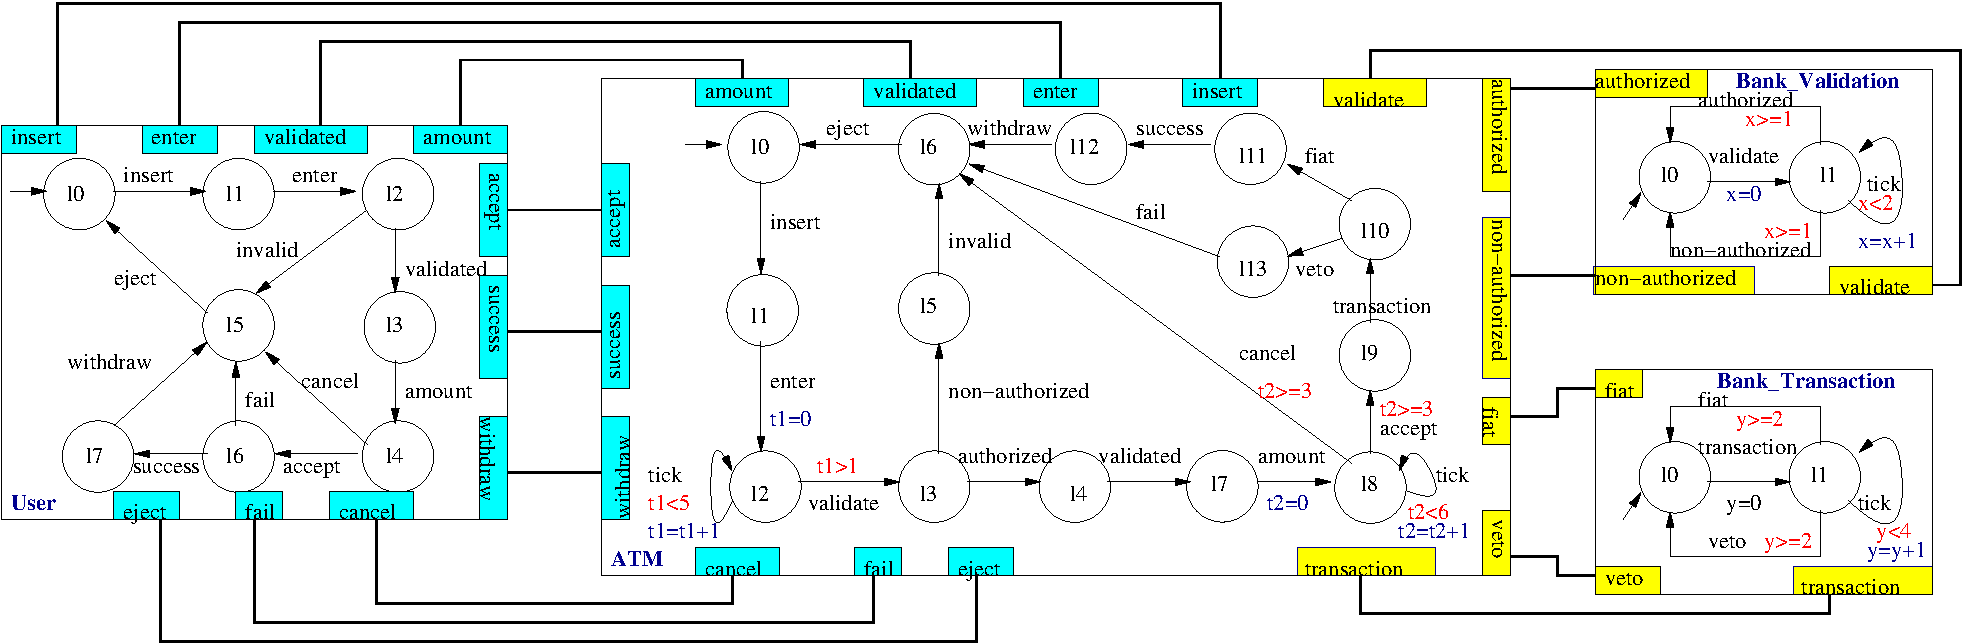
\includegraphics[width=1.0\textwidth]{figures/atm_bip.pdf}
  \resizebox{1.0\textwidth}{!}{
       \input{figures/atm_bip.pdftex_t}
  }
  \caption{Modeling of ATM system in BIP} \vspace*{-0.5cm}
  \label{fig:atm_bip}
% \end{center}
\end{figure}

The ATM starts from an idle location and waits for the user to insert his card 
and enter the confidential code. The user has $5$ time units
to enter the code before the counter expires and the card is ejected by the ATM. 
Once the code is entered, the ATM checks with the bank validation unit for 
the correctness of the code. If the code is invalid, the card is ejected
and no transaction occurs. If the code is valid, the ATM waits for the user to enter
the desired amount of money for the transaction. The time-out for entering the amount 
of money is of $6$ time units. 

Once the user enters the desired transaction amount, the ATM checks with the bank whether 
the transaction is allowed or not by communicating with the bank transaction unit.
If the transaction is approved, the money is transferred to the user and the card is ejected. 
If the transaction is rejected, the user is notified and the card is ejected. In all cases, 
the ATM goes back to the idle location waiting for any additional users. 
In our model, we assume the presence of a single bank and multiple ATMs and users. 

\begin{table}[tb]
\caption{ATM results}
\centering
\begin{tabular}{|c|c|c|c|c|c|c|c|c|c|}
\cline {2-10}
\multicolumn{1}{c|}{} &  \multicolumn{3}{c|}{Original} & \multicolumn{3}{c|}{After reduction} &  \multicolumn{3}{c|}{Time(s)} \\ \hline
ATMs & lat & and & lev & lat & and & lev & Ver. & Total& NuSMV \\ \hline
2 & 78 & 2308 & 125 & 37 & 552 & 25 & 21.83 & 26.1 & 1.4\\ \hline
3 & 102 & 3689 & 197 & 50 & 804 & 29 & 32.65 & 38.87 & 142.6 \\ \hline
4 & 146 & 5669 & 234 & 63 & 1036 & 29 & 590  & 597 & 3361 \\ \hline
\end{tabular}
\label{tb:bip:atm}
\end{table}

Table~\ref{tb:bip:atm} shows the improvement obtained by using \biptool{}
to verify the deadlock freedom of the ATM system, as compared to using the
NuSMV model checker~\cite{nusmv}.
The first column of the table shows the number of clients and ATMs in the system.
Columns \cci{lat}, \cci{and} and \cci{lev} present the number 
of latches, AND gates and logic levels in the AIG generated by \biptool{} before
and after applying reduction techniques, respectively.
We report on the verification time taken by the ABC solver to check the 
generated AIG, and the total taken to perform both synthesis (reduction) 
and verification, in addition to the time taken by NuSMV to perform verification.

With the increase in the number of users and ATMs in the system, \biptool{}  
outperforms NuSMV in terms of total verification time, reaching a speedup 
of $5.6$ for 4 users and ATMs. Additionally, \biptool{} allows developers
to make use of several reduction techniques that are able to reach an 
average of $50\%$ reduction in the size of the AIG. Note that for $2$ ATMs 
and users, NuSMV outperforms \biptool{}. This is due to the fact that when 
performing verification, ABC tries multiple verification and reduction 
algorithms before reaching a conclusive result. However, the advantage 
that \biptool{} presents can be clearly seen for larger number of ATMs and 
users. 

\section{The Quorum protocol}
The {\em Quorum} protocol is a consensus protocol proposed in~\cite{guerraoui2012speculative}
as complementary to the Paxos consensus protocol~\cite{gafni2003disk} under perfect
channel conditions. {\em Consensus} allows a set of communicating processes
(clients and servers in our case) to agree on a common value. Each of clients proposes
a value and receives a common decision value. The authors in~\cite{guerraoui2012speculative}
propose to use Quorum when no failures occur (perfect channel conditions) and 
Paxos when less than half of the servers may fail. 

The Quorum protocol operates as follows.
\begin{enumerate}
 \item Upon proposal, a client $c$ broadcasts its proposed value 
 $v$ to all servers. It also saves $v$ in its local memory and starts a local time
 $t_c$. 
 \item When a server receives a value $v$ from a client $c$, it performs
 the following check.
 \begin{itemize}
  \item It if has not sent any accept messages, it sends an accept message
  $accept(v)$ to the client $c$. 
  \item If it has already accepted value $v'$, it sends an accept message
  $accept(v')$ to the client $c$. 
 \end{itemize}
 \item If a client $c$ receives two different accept messages, it switches
 to the backup phase $switch-backup(proposal_c)$.
 \item If a client $c$ receives the same accept messages $accept(v)$ from all the servers,
 it decides on the value $v$.
 \item If a client's timer $t_c$ expires, it waits for at least
 one accept message $accept(v')$ from a server, or chooses a value $v'$
 from an already received $accept(v')$ message, and then switches to 
 the backup phase with the value $v'$. 
 \item The {\em backup} phase is an implementation of the Paxos algorithm. Quorum in this
 case has decided that the channel is not perfect. 
\end{enumerate}

We implemented the Quorum protocol in BIP, and we used \biptool{} to verify 
two invariants as defined in~\cite{guerraoui2012speculative}.
\begin{enumerate}
 \item[$Invariant_1$] If a client $c$ decides on a value $v$, then all clients 
 $c' \neq c$ that have switched, either before or after $c$, switch with the value $v$.
 \item[$Invarian_2$] If a client $c$ decides on a value $v$, then all clients
 $c' \neq c$ who decide, do so with the same value $v$. 
\end{enumerate}

Table~\ref{tb:bip:qrm} shows the results of using \biptool{} to verify the 
Quorum protocol for $2$ and $4$ clients with $2$ servers. The designs
are indexed as \cci{num\_clients}-\cci{num\_servers}-\cci{status} where 
\cci{num\_clients} is the number of clients, \cci{num\_servers} is the number of 
servers and \cci{status} is either valid (\cci{v}) or erroneous (\cci{e}).
A valid design contains no design bugs, while an errneous design is injected
with a bug. We report on the size of the AIG in terms of number of latches (\cci{lat}),
number of AND gates (\cci{and}) and logic levels (\cci{lev}) before and after
applying reduction algorithms. We also show the time taken by ABC to decide the problem, 
and the total time taken for reduction and decision procedures. 
A $\checkmark$ decision indicates that ABC proved that the property is never 
violated, \ie{} the design is valid, while a $\chi$ decision means that 
ABC was able to find a counter example that violates the property. 

\begin{table}[bt]
\caption{Quorum results}
\centering
\begin{tabular}{|c|c|c|c|c|c|c|c|c|c|}
\cline{2-9}
\multicolumn{1}{c|}{} & \multicolumn{ 3}{c|}{Original} & \multicolumn{ 3}{c|}{After reduction} & \multicolumn{ 2}{c|}{Time (s)} & \multicolumn{1}{l}{} \\ \hline
Design & lat & and & lev & lat & and & lev & Ver. & Tot. & Decision \\ \hline
2-2-v & 264 & 3614 & 105 & 66 & 641 & 29 & 240.6 & 245 & $\checkmark$\\ \hline
2-2-e & 264 & 3508 & 101 & 65 & 923 & 51 & 0.78 & 0.11 & $\chi$\\ \hline
4-2-v & 390 & 6453 & 151 & 117 & 1170 & 30 & \multicolumn{2}{c|}{58 hours}& $\checkmark$\\ \hline
4-2-e & 390 & 6305 & 145 & 117 & 1129 & 50 & 0.24 & 0.31 & $\chi$ \\ \hline
\end{tabular}
\label{tb:bip:qrm}
\end{table}

Using ABC's synthesis and reduction algorithms, \biptool{} was able to
reduce the size of the generated AIGs for all designs by a factor larger
than $50\%$. Furthermore,
\biptool{} was able to give conclusive results about all four designs, unlike
NuSMV which failed to give any decision about the designs having
$4$ clients and $2$ servers. For example, \biptool{} found a counter example for the erroneous 
design having $4$ clients and $2$ servers in $0.24 (s)$ while NuSMV failed to do
so. Figure~\ref{fig:res:counter} shows a snippet of the generated counter example for the 
erroneous design, visualized using the Gtkwave~\cite{bybell2010gtkwave} waveform viewer. 
The variables presented in the counterexample are the current control locations of
the different components in the design. 

\begin{figure}[bt]
\centering
\resizebox{1.0\textwidth}{0.25\textwidth}{
 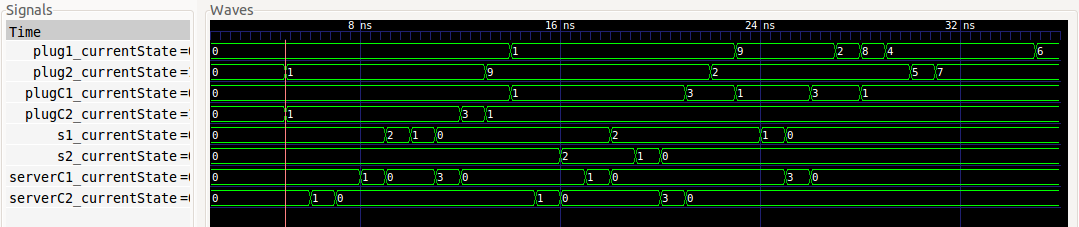
\includegraphics{figures/Quorum22CounterEx}
}
\caption{Visualization of a counter example using Gtkwave}
\label{fig:res:counter}
\end{figure}

%__________ Chapter ____________%
\chapter{Related work} \label{chap:related}
%% related work 
%% file : Literature.tex
%% Literature review for LTL synthesis

%\chapter{Related Work} \label{chap:related}

%% intro for software verification
%Ever since the success of formal verification methods in the hardware domain, researchers in the 
%software area have been trying to port the success of such techniques from hardware to software.
\section{Verification of software programs}
The need to design correct software and hardware systems has pushed researchers to design verification 
techniques and tools targeted towards software, hardware and embedded systems.
SPIN is a model checking tool targeting the verification of process interactions. It presents 
a front-end with a high level specification language called Promela, aimed at allowing users
to provide descriptions of concurrent systems or distributed algorithms~\cite{holzmann1997model}. 
SPIN accepts {\em Linear Temporal Properties} (LTL) specifications 
as input, and translates them into B\"uchi automaton using simple on-the-fly construction. 
In fact, SPIN considers the input specifications as impossible conditions, i.e. conditions that should 
never be met for correct behavior of a given system. Therefore it aims at checking whether the
language of the design and that of the specification do not intersect. If such an intersection 
exists, SPIN returns a counter example. Otherwise the design is considered to be correct. 
\mytool{} differs from SPIN in that it takes a imperative program \Pm and 
FOL precondition-postcondition pair \pair{\Pre}{\Post}, 
and translates them into an equisatisfiable AIG. On the resulting 
AIG, several reduction and proof algorithms can be applied to perform model checking, most
of which have no counterpart in SPIN.

%% Alloy and CBMC
Alloy~\cite{jackson2002alloy} and CBMC~\cite{clarke2004tool} are  tools 
that perform bounded model checking. CBMC accepts ANSI-C input code and supports
several standard C libraries. It checks for pointer operations and within bound array access, 
and allows for dynamic memory allocation using \cci{new} and \cci{malloc}. 
CBMC takes an input program and 
an unwinding bound, and generates a CNF formula that describes the behavior of the program. CBMC 
uses {\em Single Static Assignment} (SSA) transformations and loop unwinding in order to generate the appropriate CNF formula.   

Similarly, Alloy takes input structural specifications where entities can either be 
sets, functions or relations, and allows operations on these three elementary types. 
It then transforms such specifications into CNF formulae and uses SAT solvers to generate
satisfying models. Alloy differs from CBMC in that it
is aimed at generating systems that satisfy the given specifications, i.e. find models for the 
structural specifications, while CBMC is aimed at the verification of a given design against
a set of specifications. Both Alloy and CBMC transform the given problems into SAT 
problems and use an off the shelf SAT solver~\cite{goldberg2007berkmin, marques1999grasp, sorensson2005minisat} 
to try and find a model for the generated CNF formula. The model will then be a counter example
for CBMC, and a correct system for Alloy. 

Techniques based on loop unwinding and translation to CNF suffer from the rapid increase 
in the size of the generated CNF formulae with respect to the size of the input programs and
specifications, and the unwinding bounds. Additionally, the generated CNF formula may need to be
regenerated in cases where the unwinding bounds were not large enough. This iterative procedure
is costly and might require intractable resources. 

%% start here for BIP
\section{Verification of embedded systems}
The overlap between software and hardware design in embedded systems creates more challenges 
for the verification process. SystemC~\cite{systemc} is a modeling platform based on C++ that provides
design abstractions at the {\em Register Transfer Level} (RTL), behavior, and system levels. 
It aims at providing a common design environment for embedded system design and hardware-software
co-design. SystemC designers write their systems in C++ using SystemC class libraries that 
provide implementations for hardware specific objects such as concurrent modules and clocks.
Therefore the input systems can be compiled using standard C++ compilers to generate binaries
for simulation. SystemC allows for the communication between different components of a system
through the usage of ports, interfaces and channels.  

The BIP framework differs from SystemC in that it presents a dedicated language and supporting
tool-set that describes the behavior of individual system components as symbolic LTS. 
Communication between components in BIP is ensured through ports and interactions.   
BIP operates at a higher level than SystemC and does not provide support for circuit level 
constructs.

Verification techniques for SystemC and BIP make use of symbolic model checking tools. 
NuSMV2~\cite{nusmv} is a symbolic model checker that employs both 
SAT and BDD based model checking techniques. It processes an input 
describing the logical system design as a finite state machine, and a set of specifications
expressed in LTL, Computational Tree Logic (CTL) and Property Specification Language (PSL).
Given a system $\Pm$ and a set of specifications $P$, NuSMV2 first flattens $\Pm$ and $P$ by 
resolving all module instantiations and creating modules and processes, thus generating one 
synchronous design. It then performs a Boolean encoding step to eliminate all scalar variables, 
arithmetic and set operations and thus encode them as Boolean functions.   

In order to avoid the state space explosion problem, NuSMV2 performs a cone of 
influence reduction~\cite{berezin1998compositional} step in order to eliminate
non-needed parts of the flattened model and specifications. The cone of influence
reduction abstraction technique aims at simplifying the model in hand by only 
referring to variables that are of interest to the verification procedure, i.e. variables
that influence the specifications to check~\cite{clarke1999model}.

DFinder~\cite{dfinder} is an automated verification tool for checking invariants
on systems described in the BIP language. Given a BIP system \Pm and 
an invariant $\mathcal{I}$, DFinder operates  compositionally and iteratively
to compute invariants $\mathcal{X}$ of the interactions and the atomic 
components of \Pm. It then uses the Yices {\em Satisfiability Modulo
Theory} (SMT) solver~\cite{dutertre2006fast} to check for the validity 
of the formula $\mathcal{X} \land \lnot \mathcal{I} = false$. 
Additionally, DFinder checks the deadlock freedom of  \Pm by building an invariant 
$\mathcal{I}_d$ that represents the states of of \Pm in which no interactions 
are enabled, \ie{} a deadlock occurs. It then checks the for the formula
$\mathcal{X} \land \mathcal{I}_d = false$, \ie{} none of the deadlock states
are reachable in \Pm.   

Techniques based on symbolic model checking for the verification of 
BIP designs suffer from the state space explosion problem, and often 
fail to scale with the size and the complexity of the systems. 
On the other hand, DFinder does not handle data transfer between 
atomic components, thus limiting the range of practical applications 
on which it can be applied. Our technique handles data transfers and uses the wide range of synthesis 
and reduction algorithms provided by ABC to effectively reduce the size and 
the complexity of the verification problem. Most of these algorithms have no counterpart
in symbolic model checking.  


%The work in\cite{seraICSE07} takes a declarative 
%formula $\phi$ in first order logic
%(FOL) with transitive closure and a bound on the 
%universe of discourse and
%translates it to a %n equisatisfiable 
%sequential circuit expressed in VHDL. 
%It then passes the sequential circuit to a sequential 
%circuit solver and decides
%the validity of $\phi$ within the bound. 
%It scales to bounds larger than what is possible with 
%Kodkod~\cite{kodkodTJ2007}
%which translates $\phi$ into a propositional Boolean 
%formula in conjunctive
%normal form (CNF) and checks its validity with a 
%Boolean satisfiability solver. 
%
%The work in\cite{sebacASE07} translates an imperative 
%C program, with an assertion
%statement therein, and a bound on the input size, 
%into a %n equisatisfiable
%sequential circuit expressed in VHDL. 
%It then passes the sequential circuit to a 
%sequential circuit solver and decides
%the validity of the assertion within the bound. 
%It scales to bounds larger than what is possible 
%with CBMC\cite{cbmcDAC03} which
%translates the program with a bound on the input 
%size and the number of loop
%iterations into a propositional Boolean formula 
%in conjunctive normal form (CNF)
%and checks for correctness using a Boolean 
%satisfiability solver. 
%
%Our method extends the work in \cite{seraICSE07,sebacASE07} in that
%\be
%\i it supports function calls including recursion, and requires a bound on
%recursion depth only if the recursive function uses local variables, 
%\i it enables a termination guarantee check within a bound on execution
%time, it then uses the execution time bound with bounded model checking to
%decide correctness,
%\i it directly translates the program into bit level representation using {\em
%and inverted graphs} (AIG) instead of the VHDL representation that requires a
%VHDL compiler to be translated into bit level,
%\i it uses ABC~\cite{brayton2010abc}, an open source sequential circuit solver, instead of
%SixthSense~\cite{mony2004scalable} an IBM internal sequential circuit solver, 
%\i and it is an open source tool available online
%~\ref{fn:online}
%\ee
%
%%%%%%%%%%%%%%%%%%%%%%%%%%%%%%%%%%%%%%%%%%%%%%%%%%%%%%%%%%%%%%%%%%%%%%%%%%%%%%%%%%%%%%%%%%%%%%%%%%
%%% NuSVM
%NuSMV2~\cite{cimatti2002nusmv} is a symbolic model checking tool that employs both 
%satisfiability (SAT) and BDD based model checking techniques. It processes an input 
%describing the logical system design as a finite state machine, and a set of specifications
%expressed in LTL, Computational Tree Logic and Property Specification Language.
%Given a model $M$ and a set of specifications $P$, NuSMV2 first flattens $M$ and $P$ by 
%resolving all module instantiations and creating modules and processes, thus generating one 
%synchronous design. It then performs a boolean encoding step to eliminate all scalar variables, 
%arithmetic and set operations and thus encode them as boolean functions.   
%
%In order to avoid the state space explosion problem, NuSMV2 performs a cone of 
%influence reduction~\cite{berezin1998compositional} step in order to eliminate
%non-needed parts of the flattened model and specifications. The cone of influence
%reduction abstraction technique aims at simplifying the model in hand by only 
%referring to variables that are of interest to the verification procedure, i.e. variables
%that influence the specifications to check~\cite{clarke1999model}.
%%%%%%%%%%%%%%%%%%%%%%%%%%%%%%%%%%%%%%%%%%%%%%%%%%%%%%%%%%%%%%%%%%%%%%%%%%%%%%%%%%%%%%%%%%%%%%%%%%%%%
%%%%%%%%%%%%%%%%%%%%%%%%%%%%%%%%%%%%%%%%%%%%%%%%%%%%%%%%%%%%%%%%%%%%%%%%%%%%%%%%%%%%%%%%%%%%%%%%%%%%%

%\mytool{} differs from CBMC and Alloy in that it translates an input imperative program with 
%FOL specifications into a sequential circuit, encoded as an AIG. Such a representation is much 
%more succinct than CNF, and allows for much more opportunity for bit level optimizations and
%abstraction techniques that can reduce the size and the complexity of the problem. Additionally,
%it is worthy to note that network in AIG format can be easily translated in CNF formulas, so
%in the case where CNF and SAT solving outperforms sequential verification, \mytool{} can 
%perform as well as CBMC and Alloy. \mytool{} is also equipped with a debugger that allows
%a step by step inspection of the state of the each element in the code in the generated counter
%example. Such a debugger can help developers locate possible problems in their code, and even
%in their specifications.   

%%% Introduction
%Several techniques have been developed in the literature in order to synthesize LTL formulas, 
%usually describing properties that hold over real-life hardware systems and designs. These synthesis
%techniques have different targets, some aim to generate complete and correct systems based on 
%input specifications, while others are targeted at generating monitors to ensure correct
%functionality of systems through assertion checking.
%
%%% FoCs
%FoCs is an industrial tool developed at IBM research labs, targeted at generating simulation 
%checkers from formal specifications~\cite{p:Focs}. The tool's goal is to reduce, or possibly eliminate the 
%amount of human intervention in writing and maintaining functional checkers. FoCs takes input specification
%expressed in RCTL~\cite{p:rctl}, and generates formal checkers written in VHDL. These checkers
%are then linked with the original VHDL and executed on a set of test programs. The role of the formal checkers 
%is to make sure that the original design never goes into any error state. 
%
%The generation of the formal checkers from the RCTL specifications is done in three steps. First, the RCTL is 
%translated into a NFA according to the algorithm described in~\cite{p:rctl}. This NFA will have a set of error
%states, which represent the states that the design should never go into if it meets the required specifications.  
%In order to be able generate the VHDL checkers, the NFA has to be translated into a DFA, which is in turn translated
%into a VDHL process. This process will then be run alongside the original design to check for any violations of the 
%specifications. 
%
%The key drawback of FoCs' approach is that transformation algorithm generates a DFA that can be exponential 
%in the number of states of the NFA, which takes us back to the state-space explosion problem. The authors claim 
%that such a limitation does not exist in their case, since the simulation is rather sensitive to the number 
%of VHDL lines in the generated checker, which is at most quadratic in the size of the property to check. 
%Our approach differs from FoCs in that it aims at generating a DFA with auxiliary variables that is linear in 
%the size of the property, without generating any NFAs. Therefore, it can help rendering the generated VHDL checker 
%even smaller in terms of the lines of code. 
%
%%% Wring
%Daniele et. al presented an explicit state automaton based approach for model checking formulas expressed in 
%LTL~\cite{p:wring}. Explicit state refers to the fact that the automaton explicitly enumerates all of the states 
%in the system, as opposed to symbolic techniques that tend to group several states into Order Binary Decision 
%Diagrams (OBDD).
%
%In this approach,  both the system and the `negation' of the input specification are translated into automata on 
%infinite words, specifically B\"{u}chi automaton. Then, a synchronous product is applied to both of the 
%automata. If the product is empty, then the system can never go into a state that satisfies the negation 
%of the input property, i.e. the property is always satisfied and the system is correct with respect to the 
%given property. Otherwise, there exists a path that can take the system into a state that violates the 
%input specification (by satisfying its negation), and the system does not adhere to the property.  
%
%The presented algorithm, namely \texttt{`LTL2AUT'}, aims at generating a labeled B\"{u}chi automaton 
%that recognizes all of the paths that model a given LTL formula $\psi$. \texttt{LTL2AUT} in fact 
%shares its core structure with two previous algorithms, GPVW and GPVW+~\cite{p:gpvw}. Each 
%algorithm differs from the two others with the implementation of certain routines present in the 
%shared main core. The authors claim that using \texttt{LTL2AUT}, they were able to generated automata 
%with an improvement in both time (time for generation) and space (number of states) complexities, when
%compared to the other two algorithms. 
%
%%%TODO: include the rest of the literature review and compare against it


%__________ Chapter ____________%
\chapter{Conclusion} \label{chap:conclusion}
\section{Conclusion and Future Work}
\label{sec:conclusion}

In this paper we present a method for embedded system synthesis, runtime verification,
and model checking with supporting tools for the BIP framework. 
The method takes a BIP system and generates a concurrent C program with a system 
specific scheduler embedded therein. 
The concurrent C program serves as a software runtime verification simulator for the 
BIP system.
The method then take the concurrent C program and generates an AIG circuit which is an
FPGA implementation of the BIP system. 
The method applies synthesis reduction techniques using the ABC framework 
to simplify and reduce the AIG circuit
into a smaller and a less complex circuit that can be readily implemented with an 
FPGA. 
The method passes the reduced AIG circuit with a designated output that is \true
when the BIP system invariants are \true to ABC proof and model checking 
algorithms. In case ABC finds a counterexample, the methods maps the values from 
the counterexample to the original ABC system and provides the user with a debug
visualization tool. 
We successfully used the system to verify and debug medium and large case studies. 

%Currently, the system specific scheduler makes conservative decisions to avoid 
%data transfer conflicts. In the future, we plan to extend support for conflict and 
%dependency analysis so that the system specific scheduler allows for more concurrent
%behaviors. 

%For future work, we are considering several research directions. 
Currently, the system specific scheduler makes conservative decisions to avoid interaction conflicts. Two interactions are conflicting if they share a port or they are using conflicting ports of the same component. An important extension is to allow parallel execution of non-conflicting interactions using techniques presented in \cite{BonakdarpourBJQS12}. Another interesting direction is generate correct and efficient sequential circuit given real-time software (i.e., implements real-time constraints) modeled using real-time BIP \cite{AbdellatifCS13}. 




%---------------- Bibliography -------------------%
\bibliographystyle{ieeetr}
\bibliography{references/refs}



\end{document}
